\documentclass[14pt]{extarticle}

% Esto es para poder escribir acentos directamente:
\usepackage[utf8]{inputenc}
% Esto es para que el LaTeX sepa que el texto est en espaol:
\usepackage[spanish, activeacute]{babel}

% Paquetes de la AMS:
\usepackage{amsmath, amsthm, amsfonts}

\usepackage{extsizes}

\usepackage{pdflscape}
\usepackage{fontawesome}

\usepackage{graphicx}
\graphicspath{ {./images/} }

\usepackage[margin=1in]{geometry}

\usepackage{listings}
\usepackage{natbib}
\usepackage{url}
\usepackage{hyperref} % For hyperlinks in the PDF
\usepackage{multirow}
\usepackage{xifthen}
\usepackage{tabularx}

% Teoremas
%--------------------------------------------------------------------------
\newtheorem{thm}{Teorema}[section]
\newtheorem{cor}[thm]{Corolario}
\newtheorem{lem}[thm]{Lema}
\newtheorem{prop}[thm]{Proposicin}
\theoremstyle{definition}
\newtheorem{defn}[thm]{Definicin}
\theoremstyle{remark}
\newtheorem{rem}[thm]{Observacin}

% Atajos.
% Se pueden definir comandos nuevos para acortar cosas que se usan
% frecuentemente. Como ejemplo, aqu se definen la R y la Z dobles que
% suelen representar a los conjuntos de nmeros reales y enteros.
%--------------------------------------------------------------------------

\def\RR{\mathbb{R}}
\def\ZZ{\mathbb{Z}}

% De la misma forma se pueden definir comandos con argumentos. Por
% ejemplo, aqu definimos un comando para escribir el valor absoluto
% de algo ms fcilmente.
%--------------------------------------------------------------------------
\newcommand{\abs}[1]{\left\vert#1\right\vert}

\newcommand{\newtableitem}[1] {
	\multicolumn{4}{|l|}{· #1} \\
}

\newcommand{\newtableline}[1] { %55 caracteres
	\multicolumn{4}{|l|}{#1} \\
}

\newcommand{\userstory}[9]{
	\begin{center}
	\resizebox{15cm}{!} {
	\begin{tabular}{|c|c|c|c|}
    	\hline 
		\multicolumn{4}{|c|}{\textbf{#1}} \\
		\multicolumn{4}{|c|}{} \\
		\hline	
		\textbf{Identificador:} #2 & \textbf{Prioridad:} #3 & \textbf{Iteración:} #4 & \textbf{Puntos de historia:} #5 \\ 
		\hline 
		\multicolumn{4}{|l|}{\textbf{Descripción:}} \\
		#6
		\hline 
		\multicolumn{4}{|l|}{\textbf{Tareas:}} \\
		#7
		\hline 
		\multicolumn{4}{|l|}{\textbf{Pruebas de aceptación:}} \\
		#8
		\hline 
		\multicolumn{4}{|l|}{\textbf{Observaciones:}} \\
		#9
		\hline 
	\end{tabular}
	}
	\end{center}
}

\newcommand{\sprinttask}[2] {
	\multicolumn{1}{|>{\hsize=\dimexpr1\hsize+1\tabcolsep+\arrayrulewidth\relax}X|}{#1} & \multicolumn{3}{|>{\hsize=\dimexpr3\hsize+3\tabcolsep+\arrayrulewidth\relax}X|}{#2}\\
}

\newcommand{\sprint}[4]{
	\begin{center}
	\begin{tabularx}{\textwidth}{|X|X|X|X|}
    	\hline 
		\multicolumn{2}{|>{\hsize=\dimexpr2\hsize+2\tabcolsep+\arrayrulewidth\relax}X|}{\textbf{Sprint:} #1} &
		\multicolumn{2}{|>{\hsize=\dimexpr2\hsize+2\tabcolsep+\arrayrulewidth\relax}X|}{\textbf{Inicio:} #2} \\
		\hline 
		Versión & \multicolumn{3}{|>{\hsize=\dimexpr3\hsize+3\tabcolsep+\arrayrulewidth\relax}X|}{#4} \\
		\hline 
		Identificador & \multicolumn{3}{|>{\hsize=\dimexpr3\hsize+3\tabcolsep+\arrayrulewidth\relax}X|}{Historia de usuario} \\
		\hline
		#3
		\hline 
	\end{tabularx}
	\end{center}
}

% Operadores.
% Los operadores nuevos deben definirse como tales para que aparezcan
% correctamente. Como ejemplo definimos en jacobiano:
%--------------------------------------------------------------------------
\DeclareMathOperator{\Jac}{Jac}

%--------------------------------------------------------------------------
%\title{Trabajo Fin de Grado \\  TimeSeriesAnalysis: Sistema integral para análisis y predicción de series temporales.}
%\author{Javier Moreno}
\begin{document}
%\maketitle
\begin{titlepage}

\begin{center}
\vspace*{-1in}
\begin{figure}[htb]
\begin{center}

\includegraphics[scale=0.3]{ugr.png}
\end{center}
\end{figure}
ESCUELA TÉCNICA SUPERIOR DE INGENIERÍAS INFORMÁTICA Y DE TELECOMUNICACIÓN\\
\vspace*{0.15in}
DEPARTAMENTO DE COMPUTACIÓN Y SISTEMAS INTELIGENTES \\
\vspace*{0.6in}
\begin{large}
TRABAJO DE FIN DE GRADO:\\
\end{large}
\vspace*{0.2in}
\begin{Large}
\textbf{TIMESERIESANALYSIS: SISTEMA INTEGRAL PARA ANÁLISIS Y PREDICCIÓN DE SERIES TEMPORALES} \\
\end{Large}
\vspace*{0.3in}
\begin{large}
JAVIER MORENO VEGA\\
\end{large}
\vspace*{0.3in}
\rule{80mm}{0.1mm}\\
\vspace*{0.1in}
\begin{large}
TUTOR DE PROYECTO: \\
JOSÉ MANUEL BENÍTEZ SÁNCHEZ \\
\end{large}
\vspace*{2in}
\url{http://bahia.ugr.es/~jmoreno}
\vspace*{0.2in}\\
\today
\end{center}
\end{titlepage}
\newpage
\tableofcontents % índice de contenidos
\cleardoublepage
\section{Introducción}\label{sec:introduccion}
\subsection{Motivación}\label{sec:motivacion}
Las series temporales han sido, son y serán muy importantes. "Resulta difícil imaginar una rama de las ciencias en la que no aparezcan datos que puedan ser considerados como series temporales." \cite{wiki:serie_temporal}\\\\
Su definición podría ser una secuencias de datos medidos en determinados momentos y ordenados cronológicamente, pudiendo estar estos datos espaciados a intervalos iguales o desiguales. El principal uso de las series temporales es el de estudiar sus propiedades y obtener valores futuros.\\\\
Son un tipo de dato de enorme importancia en múltiples campos del conocimiento y actividad humanas. Su estudio ha preocupado a los científicos y técnicos desde hace mucho tiempo, razón por la cual existe una amplia literatura científica con propuestas de métodos para abordar su análisis (estudio de sus propiedades) y predicción (averiguar los valores futuros). Sin embargo, no existe ningún método universalmente válido pues las series pueden tener aspectos radicalmente distintos y no todos los métodos son válidos para todas. Además, en la actualidad no existe una plataforma con la que trabajar sobre series temporales sin tener que usar lenguajes de programación y eliminar la necesidad de conocimientos técnicos sobre implementación de esta funcionalidad. \\\\
Para disminuir la dificultad de un análisis de una serie temporal se ha pensado este proyecto haciendo uso de una aplicación web de un fácil uso. Desde esta aplicación web se podrá subir series temporales por los usuarios y poder aplicarles cálculos a la vez que tener una visión general.\\\\
Para analizar las series temporales haremos uso de métodos, que pueden ser transformaciones, métodos de predicción o clasificación y medidas de complejidad. Cada medida de complejidad se puede considerar como un cálculo que se hace sobre la serie temporal y devuelve un resultado numérico que identifica la complejidad de la misma. La complejidad es una medida del nivel de dificultad requerido para expresar o predecir las propiedades de un sistema \cite{article:complejidad}. En este proyecto se usa la complejidad de una serie para generar un árbol de clasificación y hacer experimentos e intentar generar una clasificación de series temporales, consiguiendo posteriormente un método automático de clasificación de series temporales y elegir el método de predicción más adecuado. \\\\
\subsection{Objetivos}\label{sec:objetivos}
El objetivo principal de este proyecto es construir un clasificador que nos asesore en la elección del método de predicción más adecuado. El conocimiento para este sistema se obtiene de analizar la base de datos de series temporales, construida para el proyecto. El análisis consiste en aplicar métodos para obtener unas medidas de cada serie temporal y poder compararlas. A estas medidas se las conoce como medidas de complejidad. Teniendo una lista de valores para cada serie se calculan grupos mediante clustering. Se obtiene la clasificación; y finalmente se calculan varios métodos de predicción sobre todas las series temporales y se selecciona de cada grupo el método con el menor error medio. La construcción de este sistema implica estudiar los principales métodos, adaptar las implementaciones disponibles o realizar implementaciones más efectivas, evaluarlos e integrarlos para que trabajen de forma cooperativa.\\\\
El objetivo secundario del proyecto es poner a disposición de los usuarios un conjunto de métodos de análisis y predicción de series temporales, que puedan ser aplicados de manera sencilla desde una aplicación web sin tener que entrar en demasiados detalles de parámetros de configuración o de la implementación de los mismos.
\subsection{Resumen del documento}\label{sec:resumen}
Esta memoria explica todo el trabajo desarrollado entrando en detalle en los módulos del sistema más importantes.\\\\ Primero se expone el análisis realizado para montar el sistema, atendiendo a: metodologías de desarrollo utilizadas, análisis de requisitos, diagramas, interfaces de usuario y las herramientas de terceros utilizadas.\\\\Posteriormente se hace una explicación detallada de la biblioteca de análisis que se ha desarrollado, explicando todos sus métodos, cada método explicado en su sección: medidas de complejidad, transformaciones, predicción y clasificación.\\\\En tercer lugar se plantea la implementación que se ha seguido entrando en detalle en lenguajes usados y realizaciones técnicas.\\\\Por último se muestran unas conclusiones, académicas y profesionales; incluyendo un resumen del trabajo desarrollado y los objetivos conseguidos.
\newpage
\section{Análisis y diseño}\label{sec:analisisydiseno}
En esta sección se explica el análisis que se ha realizado para la construcción de este proyecto junto con diagramas completos de los diversos módulos y capturas de pantalla de las interfaces de usuario.
\subsection{Metodología de desarrollo}\label{sec:metodologiadedesarrollo}
Durante el desarrollo se han usado diversas metodologías, paradigmas y patrones de arquitectura; cabe destacar como más importantes Scrum y Modelo-Vista-Controlador, esta última en la aplicación web, quse usando Angular es muy sencillo implementarla.\\\\
El modelo-vista-controlador (mvc) \cite{wiki:modelo_vista_controlador} es un patrón de arquitectura de software, el cual divide el desarrollo de un sistema en tres módulos o partes principales, separando la interfaz de usuario (vista) de la lógica (controlador) y los datos (modelo). Este patrón beneficia en la separación de conceptos lo que facilita la tarea de desarrollo y mantenimiento, además de generar una gran abstracción entre los módulos. Se ha usado en la aplicación web con Angular, aunque también se podría considerar su uso en el sistema en general ya que la abstracción realizada en módulos encajaría con mvc; siendo la vista la aplicación web, el controlador la API y el modelo las dos bases de datos y la biblioteca de métodos de análisis. Por lo tanto tendríamos una arquitectura mvc (aplicación web) que a su vez pertenece a otra arquitectura mvc (sistema completo).
\begin{center}
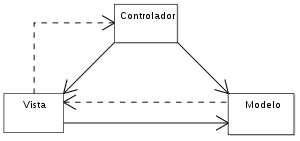
\includegraphics{modelo_vista_controlador.png}
\end{center}
La metodología de desarrollo usada ha sido Scrum \cite{wiki:scrum} que es una metodología de desarrollo ágil caracterizada por tener una estrategia de desarrollo incremental y una ejecución completa del producto por intervalos, equipos de desarrollo auto organizados y solapamiento de las diferentes fases del desarrollo. Cada iteración del desarrollo es un "sprint" y al finalizar cada uno se crea un incremento de software utilizable, la duración de estos suele ser entre 2 y 3 semanas.\\\\
Los roles principales en scrum son: Product owner (representa la voz del client), scrum master (elimina obstáculos dentro del equipo y se encarga de que funcione scrum) y el equipo de desarrollo (puede estar formado por desarrolladores de software, testers, documentadores, etc). Cada equipo debe tener estos roles bien definidos.\\\\
También se realizan diversas reuniones: Daily scrum (reuniones diarias para ver como va el desarrollo), planificación (como su propio nombre indica planificar el desarrollo que se realizará en los próximos sprints), revisión del sprint (presentar el trabajo desarrollado) y retrospectiva del sprint (los miembros del equipo proponen mejorar y problemas que han podido ocurrir durante el sprint).\\\\
Todo el desarrollo que se va a realizar se agrupa en documentos llamados historias de usuario, cada historia de usuario contiene una funcionalidad completa y bien definida, y estas se dividen a su vez en tareas de desarrollo. Y todas las historias el equipo las tiene que puntuar con puntos de historia que deben seguir la sucesión de Fibonacci \cite{wiki:fibonacci} (0, 1, 1, 2, 3, 5, 8, 13, ...), esto es indicativo para ver la dificultad de cada historia, a mayor dificultad mayor puntuación.\\\\
Los elementos usados para el desarrollo son: product backlog (agrupación de todas las historias de usuario del proyecto), sprint backlog (subconjunto de historias de usuario que se realizarán, o se intentaran, en el sprint), burn down chart (gráfica que muestra el progreso del desarrollo conforme se van acabando historias de usuario y reduciendo el número de puntos de historia restantes).\\\\
La elección de esta metodología es debido a tener experiencia propia por haber trabajado profesionalmente con ella, pero sobre todo el que ofrezca un desarrollo iterativo e incremental evitando el seguimiento de un estricto plan, adaptándose de forma continua a las circunstancias del proyecto.
\begin{center}
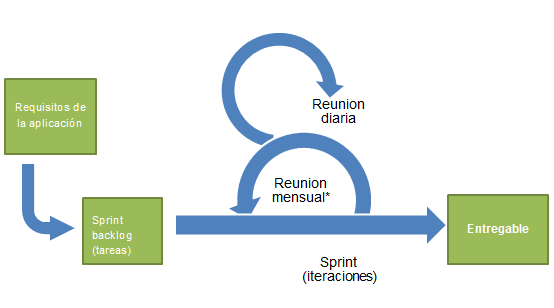
\includegraphics{Scrum.png}
\end{center}
\subsection{Análisis de requisitos}\label{sec:analisisderequisitos}
En esta sección se realiza el análisis de requisitos del sistema y como se hace uso de Scrum los casos de uso se estructuran en historias de usuario y se incluyen en el backlog.\\\\El desarrollo se ha realizado en dos fases con un periodo de 1 mes entre ambas donde se realizó investigación.\\\\Después de un tiempo de estudio de los requisitos y la funcionalidad que debía tener el sistema se han obtenido las siguientes historias de usuario que formaran el product backlog en la primera fase de desarrollo.

Consideraciones:
\begin{itemize}
	\item Usuario anónimo: Es considerado como un usuario que no ha iniciado sesión en la aplicación.
	\item Usuario registrado: Es considerado como un usuario que ha iniciado sesión correctamente en la aplicación.
	\item Usuario: Es considerado como un usuario general pudiendo haber iniciado sesión o no.
\end{itemize}

\userstory {Crear una nueva cuenta de usuario}
{HU001}{1}{1}{5}
{\newtableline {Como usuario anónimo quiero poder crear una nueva cuenta.}}
{ %Tareas
	\newtableitem {Construir la capa de datos en el servidor para crear }
		\newtableline {usuarios (base de datos SQL).}
	\newtableitem {Construir método en la API para crear nuevas cuentas de usuario.}
	\newtableitem {Construir método en la API para validar datos.}
	\newtableitem {Construir la interfaz de usuario para crear la cuenta.}
	\newtableitem {Implementar conexiones con la API desde el cliente.}
	\newtableitem {Gestionar las diferentes respuestas en el cliente.}
}
{ %Pruebas de aceptación
	\newtableitem {Crear cuenta de usuario correctamente.}
	\newtableitem {Validar datos correctamente.}
	\newtableitem {Mostrar diferentes errores en el cliente.}
}
{ %Observaciones

}

\userstory {Iniciar sesión}
{HU002}{1}{2}{5}
{\newtableline {Como usuario anónimo quiero poder iniciar sesión.}}
{ %Tareas
	\newtableitem {Construir método en la API para iniciar sesión como usuario.}
	\newtableitem {Construir la interfaz de usuario para iniciar sesión.}
	\newtableitem {Implementar conexiones con la API desde el cliente.}
	\newtableitem {Gestionar las diferentes respuestas en el cliente.}
}
{ %Pruebas de aceptación
	\newtableitem {Iniciar sesión correctamente.}
	\newtableitem {Mostrar diferentes errores en el cliente.}
}
{ %Observaciones
	\newtableline {Depende de HU001 para poder crear la cuenta de usuario} 
	\newtableline{ antes de iniciar sesión.}
}

\userstory {Subir serie temporal}
{HU003}{1}{2}{8}
{\newtableline {Como usuario registrado quiero poder subir/crear una nueva}
\newtableline{ serie temporal pública o privada.}}
{ %Tareas
	\newtableitem {Construir la capa de datos en el servidor para crear}
		\newtableline { series temporales (base de datos SQL).}
	\newtableitem {Construir la capa de datos en el servidor para crear}
		\newtableline { series temporales (base de datos InfluxDB).}
	\newtableitem {Añadir método a la biblioteca de métodos R para calcular}
		\newtableline { propiedades de una serie temporal}
	\newtableitem {Construir método en la API para crear series temporales}
		\newtableline { llamando al método de la biblioteca R para calcular}
		\newtableline { propiedades de la serie temporal.}
	\newtableitem {Construir la interfaz de usuario para subir series temporales.}
	\newtableitem {Construir método en la API para validar datos.}
	\newtableitem {Implementar conexiones con la API desde el cliente.}
	\newtableitem {Gestionar las diferentes respuestas en el cliente.}
}
{ %Pruebas de aceptación
	\newtableitem {Subir serie temporal correctamente.}
	\newtableitem {Mostrar diferentes errores en el cliente.}
}
{ %Observaciones
	\newtableline {Depende de HU001 para poder crear las series temporales} 
	\newtableline{ habiendo iniciado sesión.}
}

\userstory {Listado de series temporales públicas}
{HU004}{1}{3}{2}
{\newtableline {Como usuario quiero poder ver un listado de las series}
\newtableline{ temporales públicas almacenadas.}}
{ %Tareas
	\newtableitem {Construir método en la API para devolver un listado de series}
		\newtableline { temporales públicas almacenadas.}
	\newtableitem {Construir la interfaz de usuario para ver listado de series temporales.}
	\newtableitem {Implementar conexiones con la API desde el cliente.}
	\newtableitem {Gestionar las diferentes respuestas en el cliente.}
}
{ %Pruebas de aceptación
	\newtableitem {Listar series temporales públicas almacenadas.}
	\newtableitem {Mostrar diferentes errores en el cliente.}
}
{ %Observaciones
	\newtableline {Depende de HU003 para tener series temporales almacenadas.} 
}

\userstory {Listado de series temporales de usuario}
{HU005}{2}{3}{3}
{\newtableline {Como usuario registrado quiero poder ver un listado}
\newtableline{ de mis series temporales.}}
{ %Tareas
	\newtableitem {Construir método en la API para devolver un listado de series}
		\newtableline { temporales de un usuario almacenadas.}
	\newtableitem {Construir la interfaz de usuario para ver listado de series}
		\newtableline { temporales propias almacenadas.}
	\newtableitem {Implementar conexiones con la API desde el cliente.}
	\newtableitem {Gestionar las diferentes respuestas en el cliente.}
}
{ %Pruebas de aceptación
	\newtableitem {Listar series temporales de un usuario almacenadas.}
	\newtableitem {Mostrar diferentes errores en el cliente.}
}
{ %Observaciones
	\newtableline {Depende de HU003 para tener series temporales almacenadas.} 
}

\userstory {Mostrar serie temporal}
{HU006}{1}{3}{3}
{
	\newtableline {Como usuario quiero poder ver una serie temporal.}
}
{ %Tareas
	\newtableitem {Construir método en la API para devolver una serie}
		\newtableline { temporal sin valores.}
	\newtableitem {Construir la interfaz de usuario para ver una serie temporal}
	\newtableitem {Implementar conexiones con la API desde el cliente.}
	\newtableitem {Gestionar las diferentes respuestas en el cliente.}
}
{ %Pruebas de aceptación
	\newtableitem {Mostrar serie temporal.}
	\newtableitem {Mostrar diferentes errores en el cliente.}
}
{ %Observaciones
	\newtableline {Depende de HU003 para tener series temporales almacenadas.} 
}

\userstory {Mostrar gráfica de serie temporal}
{HU007}{1}{4}{3}
{
	\newtableline {Como usuario quiero poder ver una gráfica de la serie temporal.}
}
{ %Tareas
	\newtableitem {Modificar método de la API para devolver una serie}
		\newtableline { temporal con valores.}
	\newtableitem {Construir la interfaz de usuario para ver una gráfica de la}
		\newtableline { serie temporal}
	\newtableitem {Gestionar las diferentes respuestas en el cliente.}
}
{ %Pruebas de aceptación
	\newtableitem {Mostrar gráfica de la serie temporal.}
	\newtableitem {Mostrar diferentes errores en el cliente.}
}
{ %Observaciones
	\newtableline {Depende de HU006 para poder acceder a la serie temporal.} 
}

\userstory {Mostrar características principales de una serie temporal}
{HU008}{1}{4}{2}
{
	\newtableline {Como usuario quiero poder ver las características principales }
	\newtableline { definidas y obtenidas de una serie temporal.}
}
{ %Tareas
	\newtableitem {Modificar la interfaz de usuario para ver nuevas propiedades}
		\newtableline { de una serie temporal}
	\newtableitem {Gestionar las diferentes respuestas en el cliente.}
}
{ %Pruebas de aceptación
	\newtableitem {Mostrar propiedades de la serie temporal.}
	\newtableitem {Mostrar diferentes errores en el cliente.}
}
{ %Observaciones
	\newtableline {Depende de HU006 para poder acceder a la serie temporal.} 
}

\userstory {Mostrar métodos de análisis de una serie temporal}
{HU009}{1}{4}{3}
{
	\newtableline {Como usuario quiero poder ver un listado}
	\newtableline { de selección con los tipos de análisis de}
	\newtableline { series temporales disponibles.}
}
{ %Tareas
	\newtableitem {Añadir funcionalidad a la biblioteca de métodos R para}
		\newtableline { obtener los métodos de análisis.}
	\newtableitem {Añadir funcionalidad a la API para conectar con la biblioteca}
		\newtableline { de métodos R.}
	\newtableitem {Modificar la interfaz de usuario para mostrar un selector con}
		\newtableline { los tipos de métodos de análisis disponibles.}
	\newtableitem {Gestionar las diferentes respuestas en el cliente.}
}
{ %Pruebas de aceptación
	\newtableitem {Mostrar selector con los diferentes métodos de análisis.}
	\newtableitem {Mostrar diferentes errores en el cliente.}
}
{ %Observaciones
	\newtableline {Depende de HU006 para poder acceder a la interfaz}
	\newtableline { de la serie temporal.} 
}

\userstory {Mostrar selector de tipo de serie temporal a la que aplicar método}
{HU010}{1}{5}{3}
{
	\newtableline {Como usuario quiero poder ver un listado}
	\newtableline { de las series temporales a las que aplicar}
	\newtableline { los métodos de análisis}
}
{ %Tareas
	\newtableitem {Añadir funcionalidad a la biblioteca de métodos R para}
		\newtableline { obtener un listado de métodos de transformación.}
	\newtableitem {Añadir funcionalidad a la API para conectar con la biblioteca}
		\newtableline { de métodos R.}
	\newtableitem {Modificar la interfaz de usuario para mostrar un selector con}
		\newtableline { los tipos de series temporales transformadas y la original.}
	\newtableitem {Gestionar las diferentes respuestas en el cliente.}
}
{ %Pruebas de aceptación
	\newtableitem {Mostrar selector con las diferentes series temporales.}
	\newtableitem {Mostrar diferentes errores en el cliente.}
}
{ %Observaciones
	\newtableline {Depende de HU009 para añadir el selector del tipo de serie temporal.} 
}

\userstory {Aplicar métodos de transformación a una serie temporal}
{HU011}{1}{6}{5}
{
	\newtableline {Como usuario quiero poder aplicar transformaciones a}
	\newtableline { una serie temporal original o transformada y}
	\newtableline { poder ver una gráfica con la serie transformada.}
}
{ %Tareas
	\newtableitem {Añadir funcionalidad a la biblioteca de métodos R para}
		\newtableline { aplicar métodos de transformación a una serie temporal.}
	\newtableitem {Añadir funcionalidad a la API para conectar con la biblioteca}
		\newtableline { de métodos R.}
	\newtableitem {Modificar la interfaz de usuario para mostrar un}
		\newtableline { selector con los diferentes métodos de transformación.}
	\newtableitem {Modificar la interfaz de usuario para aplicar métodos}
		\newtableline { de transformación a una serie temporal.}
	\newtableitem {Modificar la interfaz de usuario para mostrar }
		\newtableline { la gráfica de la transformación de una serie temporal.}
	\newtableitem {Gestionar las diferentes respuestas en el cliente.}
}
{ %Pruebas de aceptación
	\newtableitem {Mostrar gráfica de transformación de la serie temporal.}
	\newtableitem {Mostrar diferentes errores en el cliente.}
}
{ %Observaciones
	\newtableline {Depende de HU010 para aplicar métodos a la serie temporal.} 
}

\userstory {Aplicar medidas de complejidad a una serie temporal}
{HU012}{1}{6}{5}
{
	\newtableline {Como usuario quiero poder aplicar medidas de}
	\newtableline { complejidad a una serie temporal original o }
	\newtableline { transformada y poder ver los resultados.}
}
{ %Tareas
	\newtableitem {Añadir funcionalidad a la biblioteca de métodos R para}
		\newtableline { obtener un listado de medidas de complejidad.}
	\newtableitem {Añadir funcionalidad a la biblioteca de métodos R para}
		\newtableline { aplicar medidas de complejidad a una serie temporal}
	\newtableitem {Añadir funcionalidad a la API para conectar con la biblioteca}
		\newtableline { de métodos R.}
	\newtableitem {Modificar la interfaz de usuario para mostrar un}
		\newtableline { selector con las diferentes medidas de complejidad.}
	\newtableitem {Modificar la interfaz de usuario para aplicar medidas}
		\newtableline { de complejidad a una serie temporal}
	\newtableitem {Modificar la interfaz de usuario para mostrar los resultados}
	\newtableitem {Gestionar las diferentes respuestas en el cliente.}
}
{ %Pruebas de aceptación
	\newtableitem {Mostrar resultados de complejidad de la serie temporal.}
	\newtableitem {Mostrar diferentes errores en el cliente.}
}
{ %Observaciones
	\newtableline {Depende de HU010 para aplicar métodos a la serie temporal.} 
}

\userstory {Aplicar métodos de predicción a una serie temporal}
{HU013}{1}{6}{5}
{
	\newtableline {Como usuario quiero poder aplicar métodos de}
	\newtableline { predicción a una serie temporal original o}
	\newtableline { tranformada y poder ver una gráfica con la}
	\newtableline { predicción y demás resultados.}
}
{ %Tareas
	\newtableitem {Añadir funcionalidad a la biblioteca de métodos R para}
		\newtableline { obtener un listado de métodos de predicción.}
	\newtableitem {Añadir funcionalidad a la biblioteca de métodos R para}
		\newtableline { aplicar métodos de predicción a una serie temporal}
	\newtableitem {Añadir funcionalidad a la API para conectar con la biblioteca}
		\newtableline { de métodos R.}
	\newtableitem {Modificar la interfaz de usuario para mostrar un}
		\newtableline { selector con los diferentes métodos de predicción.}
	\newtableitem {Modificar la interfaz de usuario para aplicar métodos}
		\newtableline { de predicción a una serie temporal}
	\newtableitem {Modificar la interfaz de usuario para mostrar los resultados}
		\newtableline { añadiendo una gráfica con los valores futuros.}
	\newtableitem {Gestionar las diferentes respuestas en el cliente.}
}
{ %Pruebas de aceptación
	\newtableitem {Mostrar resultados de predicción de la serie temporal}
		\newtableline { incluyendo una gráfica con los valores futuros.}
	\newtableitem {Mostrar diferentes errores en el cliente.}
}
{ %Observaciones
	\newtableline {Depende de HU010 para aplicar métodos a la serie temporal.} 
}

\userstory {Aplicar métodos de clasificación a una serie temporal}
{HU014}{1}{6}{5}
{
	\newtableline {Como usuario quiero poder aplicar métodos de clasificación}
	\newtableline { a una serie temporal original o tranformada y poder ver}
	\newtableline { los resultados.}
}
{ %Tareas
	\newtableitem {Añadir funcionalidad a la biblioteca de métodos R para}
		\newtableline { obtener un listado de métodos de clasificación.}
	\newtableitem {Añadir funcionalidad a la biblioteca de métodos R para}
		\newtableline { aplicar métodos de clasificación a una serie temporal}
	\newtableitem {Añadir funcionalidad a la API para conectar con la biblioteca}
		\newtableline { de métodos R.}
	\newtableitem {Modificar la interfaz de usuario para mostrar un}
		\newtableline { selector con los diferentes métodos de clasificación.}
	\newtableitem {Modificar la interfaz de usuario para aplicar métodos}
		\newtableline { de clasificación a una serie temporal}
	\newtableitem {Modificar la interfaz de usuario para mostrar los resultados.}
	\newtableitem {Gestionar las diferentes respuestas en el cliente.}
}
{ %Pruebas de aceptación
	\newtableitem {Mostrar resultados de clasificación de la serie temporal.}
	\newtableitem {Mostrar diferentes errores en el cliente.}
}
{ %Observaciones
	\newtableline {Depende de HU010 para aplicar métodos a la serie temporal.} 
}

\userstory {Mostrar series temporales privadas a sus usuarios}
{HU015}{2}{3}{3}
{
	\newtableline {Como usuario registrado quiero poder acceder a mis series temporales}
	\newtableline { privadas.}
}
{ %Tareas
	\newtableitem {Añadir autentificación en la API al intentar acceder a series}
		\newtableline { temporales privadas.}
	\newtableitem {Añadir mensaje de error en la interfaz al acceder sin permisos}
		\newtableline { a una serie temporal privada.}
}
{ %Pruebas de aceptación
	\newtableitem {Mostrar serie temporal privada si es del usuario.}
	\newtableitem {Mostrar diferentes errores en el cliente.}
}
{ %Observaciones
	\newtableline {Depende de HU003 para tener series temporales almacenadas.}
}

\userstory {Acceder a perfil de usuario registrado}
{HU016}{3}{3}{3}
{
	\newtableline {Como usuario registrado quiero poder acceder a mi perfil.}
}
{ %Tareas
	\newtableitem {Añadir menú de usuario a la pantalla de análisis}
	\newtableitem {Añadir método de obtener usuario en la API.}
	\newtableitem {Construir interfaz de edición de perfil de usuario}
		\newtableline { registrado.}
	\newtableitem {Añadir a la interfaz el listado de las series}
		\newtableline { temporales del usuario.}
	\newtableitem {Implementar conexiones con la API desde el cliente.}
	\newtableitem {Gestionar las diferentes respuestas en el cliente.}
}
{ %Pruebas de aceptación
	\newtableitem {Mostrar correctamente perfil de usuario registrado.}
	\newtableitem {Mostrar diferentes errores en el cliente.}
}
{ %Observaciones
	\newtableline {Depende de HU001 para poder iniciar sesión.} 
}

\userstory {Editar perfil de usuario registrado}
{HU017}{3}{3}{3}
{
	\newtableline {Como usuario registrado quiero poder editar mi perfil.}
}
{ %Tareas
	\newtableitem {Añadir método con autentificación en la API para poder}
		\newtableline { modificar datos de usuario registrado}
	\newtableitem {Añadir método de validación de datos en la API.}
	\newtableitem {Construir interfaz de edición de perfil de usuario}
		\newtableline { registrado.}
	\newtableitem {Implementar conexiones con la API desde el cliente.}
	\newtableitem {Gestionar las diferentes respuestas en el cliente.}
}
{ %Pruebas de aceptación
	\newtableitem {Modificar correctamente perfil de usuario registrado.}
	\newtableitem {Mostrar diferentes errores en el cliente.}
}
{ %Observaciones
	\newtableline {Depende de HU001 para poder iniciar sesión.} 
}Una vez se han obtenido las historias de usuario es necesario hacer una aproximación de la velocidad de desarrollo para hacer las divisiones de Sprint.\\\\
La duración de un Sprint en el proyecto será de dos semanas, por tanto se tienen 15 días de desarrollo por Sprint. Y tendremos como velocidad estimada por Sprint de 8 puntos de historia.\\\\
Considerando que se tienen 63 puntos de historia del proyecto completo y la velocidad de desarrollo se obtienen un total de 8 Sprint.\\\\
A continuación se muestran las historias de usuario divididas por Sprint, para la primera fase, desarrollándose primero las que más prioridad tienen. Con la finalización de estos primeros 8 Sprint obtendremos la versión Alpha-2.0.0 del producto.\\\\

\sprint {1}{25/07/2016}
{
	\sprinttask {HU001}{Crear una nueva cuenta de usuario}
	\sprinttask {HU002}{Iniciar sesión}
}{Alpha-2.0.0}

\sprint {2}{08/08/2016}
{
	\sprinttask {HU003}{Subir serie temporal}
}{Alpha-2.0.0}

\sprint {3}{22/08/2016}
{
	\sprinttask {HU004}{Listado de series temporales públicas}
	\sprinttask {HU006}{Mostrar serie temporal}
	\sprinttask {HU007}{Mostrar gráfica de serie temporal}
}{Alpha-2.0.0}

\sprint {4}{05/09/2016}
{
	\sprinttask {HU008}{Mostrar características principales de una serie temporal}
	\sprinttask {HU009}{Mostrar métodos de análisis de una serie temporal}
	\sprinttask {HU010}{Mostrar selector de tipo de serie temporal a la que aplicar método}
}{Alpha-2.0.0}

\sprint {5}{19/09/2016}
{
	\sprinttask {HU005}{Listado de series temporales de usuario}
	\sprinttask {HU011}{Aplicar métodos de transformación a una serie temporal}
}{Alpha-2.0.0}

\sprint {6}{03/10/2016}
{
	\sprinttask {HU012}{Aplicar medidas de complejidad a una serie temporal}
	\sprinttask {HU015}{Mostrar series temporales privadas a sus usuarios}
}{Alpha-2.0.0}

\sprint {7}{17/10/2016}
{
	\sprinttask {HU013}{Aplicar métodos de predicción a una serie temporal}
	\sprinttask {HU016}{Acceder a perfil de usuario registrado}
}{Alpha-2.0.0}

\sprint {8}{31/10/2016}
{
	\sprinttask {HU014}{Aplicar métodos de clasificación a una serie temporal}
	\sprinttask {HU017}{Editar perfil de un usuario registrado}
}{Alpha-2.0.0}

La segunda fase del desarrollo comienza un mes depués de la finalización de la primera. A continuación se muestran las historias obtenidas para esta fase.

\userstory {Misceláneos 1}
{HU018}{1}{1}{5}
{
	\newtableline {Historia de usuario para refactorizar y dividir paquete R }
	\newtableline {TimeSerie en varios paquetes más pequeños.}
}
{ %Tareas
	\newtableitem {Crear paquete R DataUtils}
	\newtableitem {Crear paquete R TimeSeries}
	\newtableitem {Crear paquete R TimeSeriesAnalysis}
	\newtableitem {Crear paquete R Clustering}
}
{ %Pruebas de aceptación
	\newtableitem {Tests funcionando en paquete DataUtils.}
	\newtableitem {Tests funcionando en paquete TimeSeries.}
	\newtableitem {Tests funcionando en paquete TimeSeriesAnalysis.}
	\newtableitem {Tests funcionando en paquete Clustering.}
	\newtableitem {TimeSeriesAnalysisWebApi sigue funcionando correctamente.}
}
{ %Observaciones
}

\userstory {Misceláneos 2}
{HU019}{3}{1}{3}
{
	\newtableline {Historia de usuario para refactorización y mejoras.}
}
{ %Tareas
	\newtableitem {Mejorar automatización de Dockers.}
}
{ %Pruebas de aceptación
	\newtableitem {Mantener funcionamiento correcto de base de datos de series temporales.}
	\newtableitem {Mantener funcionamiento correcto de script de gestión de Docker.}
}
{ %Observaciones
}

\userstory {Misceláneos 3}
{HU020}{2}{1}{3}
{
	\newtableline {Historia de usuario para refactorizar las URIs de }
	\newtableline {TimeSeriesAnalysisWebApi.}
}
{ %Tareas
	\newtableitem {Mejorar URIs de TimeSeriesAnalysisWebApi.}
	\newtableitem {Mejorar API y URIS WebApp.}
}
{ %Pruebas de aceptación
	\newtableitem {Mantener funcionamiento correcto de la API.}
}
{ %Observaciones
}

\userstory {Misceláneos 4}
{HU021}{2}{1}{3}
{
	\newtableline {Historia de usuario para refactorización y mejoras.}
}
{ %Tareas
	\newtableitem {Añadir PHP tests}
}
{ %Pruebas de aceptación
	\newtableitem {Mantener funcionamiento correcto de la API.}
	\newtableitem {Mantener funcionamiento correcto de la App.}
}
{ %Observaciones
}

\userstory {Clasificar series temporales (Mejoras)}
{HU022}{1}{1}{8}
{
	\newtableline {Como usuario quiero poder clasificar series }
	\newtableline {temporales correctamente según una clasificación.}
}
{ %Tareas
	\newtableitem {Añadir InfluxDB Docker.}
	\newtableitem {Mejorar lectura de TimeSeries R (Date) }
		\newtableline{/ Leer desde DB TimeSeries R}
	\newtableitem {Scripts de investigación}
}
{ %Pruebas de aceptación
	\newtableitem {Clasificar correctamente una serie temporal.}
}
{ %Observaciones
}

\userstory {Documentación General (DOC)}
{HU023}{3}{5}{3}
{
	\newtableline {Historia de usuario para añadir la }
	\newtableline {documentación restante a la memoria.}
}
{ %Tareas
	\newtableitem {Añadir youtrack y teamcity al software}
	\newtableitem {Explicar gestión de Docker's.}
	\newtableitem {Actualizar diagramas.}
	\newtableitem {Conclusiones académicas}
}
{ %Pruebas de aceptación
	\newtableitem {}
}
{ %Observaciones
}

\userstory {Clasificación de serie temporal (DOC)}
{HU024}{1}{2}{3}
{
	\newtableline {Historia de usuario para añadir }
	\newtableline {la documentación acerca de clasificar series temporales a la memoria.}
}
{ %Tareas
	\newtableitem {Explicar investigación clasificación}
	\newtableitem {Añadir información a Home de WebApp}
}
{ %Pruebas de aceptación
	\newtableitem {}
}
{ %Observaciones
	\newtableline {Depende de HU023 debido a que es necesario }
	\newtableline {el desarrollo antes de la documentación.}
}

\userstory {Medidas de complejidad (DOC)}
{HU030}{1}{1}{3}
{
	\newtableline {Historia de usuario para añadir la documentación }
	\newtableline {acerca de medidas de complejidad a la memoria.}
}
{ %Tareas
	\newtableitem {Descripción de medidas de complejidad.}
	\newtableitem {Añadir información a Home de WebApp.}
}
{ %Pruebas de aceptación
	\newtableitem {}
}
{ %Observaciones
}De nuevo se vuelven a dividir las historias de usuario por Sprint. En esta fase cada vez que se finalize un Sprint se procederá a liberar una nueva versión del producto ya que como se comenta en el apartado de software usado durante el desarrollo ahora haremos uso de un servidor de integración continua con ejecución de Tests y Build.\\\\
\sprint {9}{12/12/2016}
{
	\sprinttask {HU035}{Medidas de complejidad (DOC)}
	\sprinttask {HU024}{Clasificación de serie temporal (DOC)}	
}{Alpha-2.1.0}

\sprint {10}{26/12/2016}
{
	\sprinttask {HU022}{Clasificar series temporales (Mejoras)}
}{Alpha-2.2.0}

\sprint {11}{09/01/2017}
{
	\sprinttask {HU018}{Misceláneos 1}
	\sprinttask {HU020}{Misceláneos 3}
	\sprinttask {HU025}{Subir serie temporal (Mejoras)}
}{Alpha-2.3.0}

\sprint {12}{23/01/2017}
{
	\sprinttask {HU026}{Listar series temporales con paginación}
	\sprinttask {HU019}{Misceláneos 2}
}{Beta-1.0.0}

\sprint {13}{06/02/2017}
{
	\sprinttask {HU023}{Documentación General (DOC)}
}{Beta-1.0.0 (No hay desarrollo)}

\newpage
\subsection{Diagramas}\label{sec:diagramas}
En esta sección se mostrarán los diagramas de diseño utilizados en el sistema. Primero se va a mostrar un diagrama sobre el sistema completo.

\begin{center}
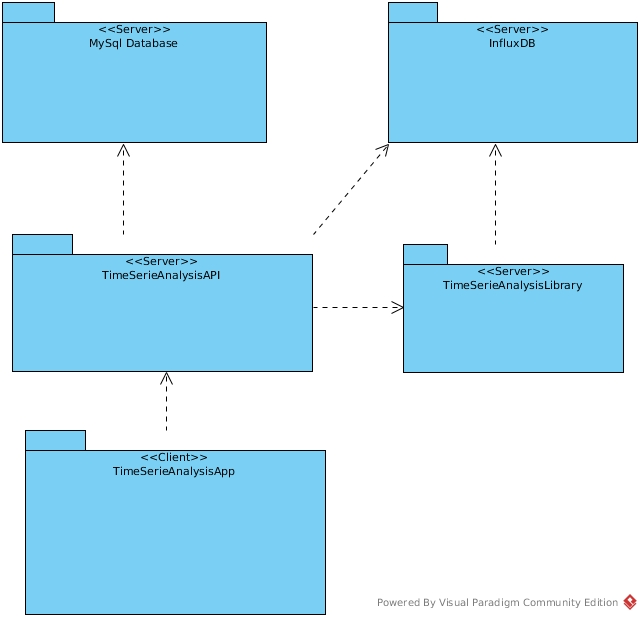
\includegraphics[scale=0.7]{DiagramaDePaquetes.jpg}
Imagen 1: Diagrama de módulos del sistema completo.
\end{center}

\newpage
A continuación se mostrarán todos los diagramas del sistema comenzando desde la base de datos SQL, y continuando con todos los módulos del sistema, en el caso de TimeSeriesAnalysisLibrary también se mostraran los subdiagramas de clases de sus paquetes R:
\begin{itemize}
	\item TimeSeriesAnalysisLibrary
	\item TimeSeriesAnalysisAPI
	\item TimeSeriesAnalysisApp
\end{itemize}

\begin{center}
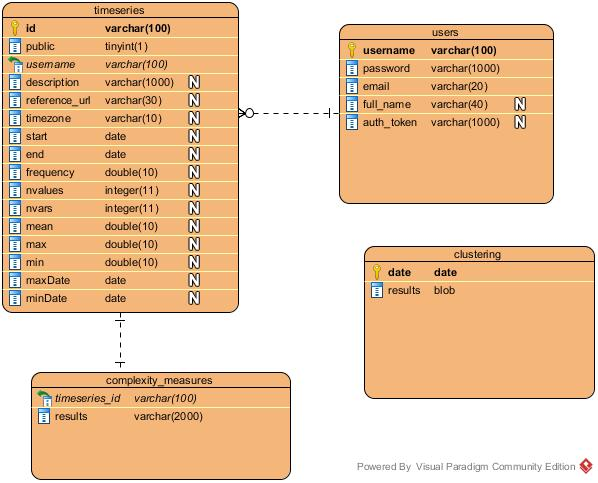
\includegraphics[scale=0.7]{Database.jpg}
\\Imagen 2: Diagrama de datos SQL
\end{center}

\begin{landscape}
	\begin{center}
	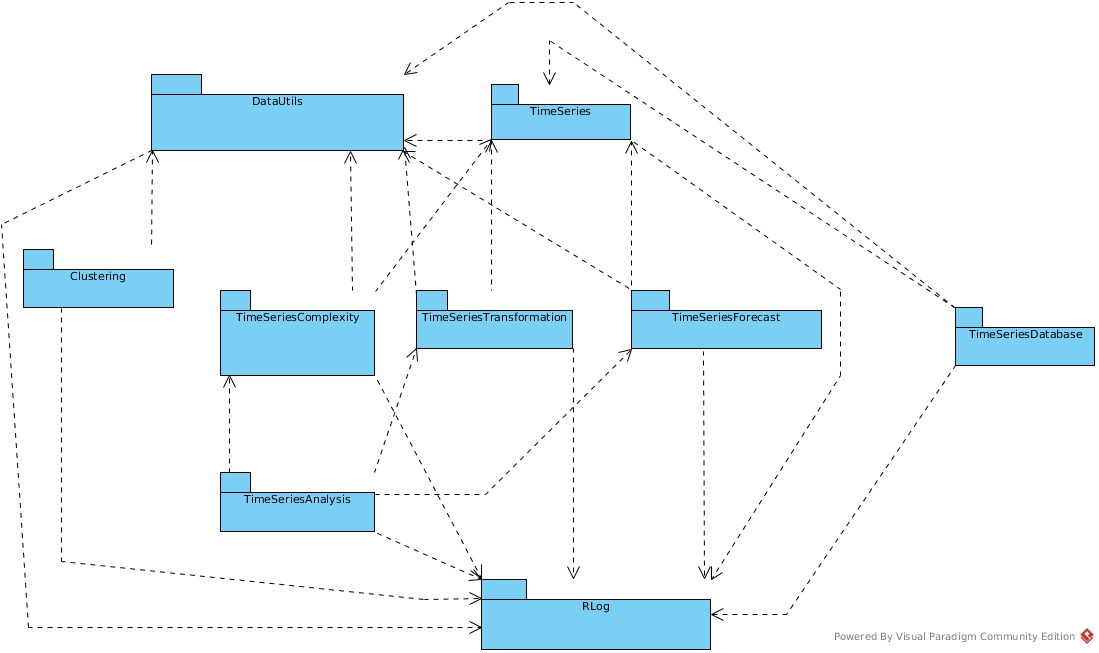
\includegraphics[scale=0.6]{TimeSeriesAnalysisLibrary.jpg}
	\\Imagen 3: Diagrama de paquetes R (TimeSeriesAnalysisLibrary)
	\end{center}
\end{landscape}

\begin{landscape}
	\begin{center}
	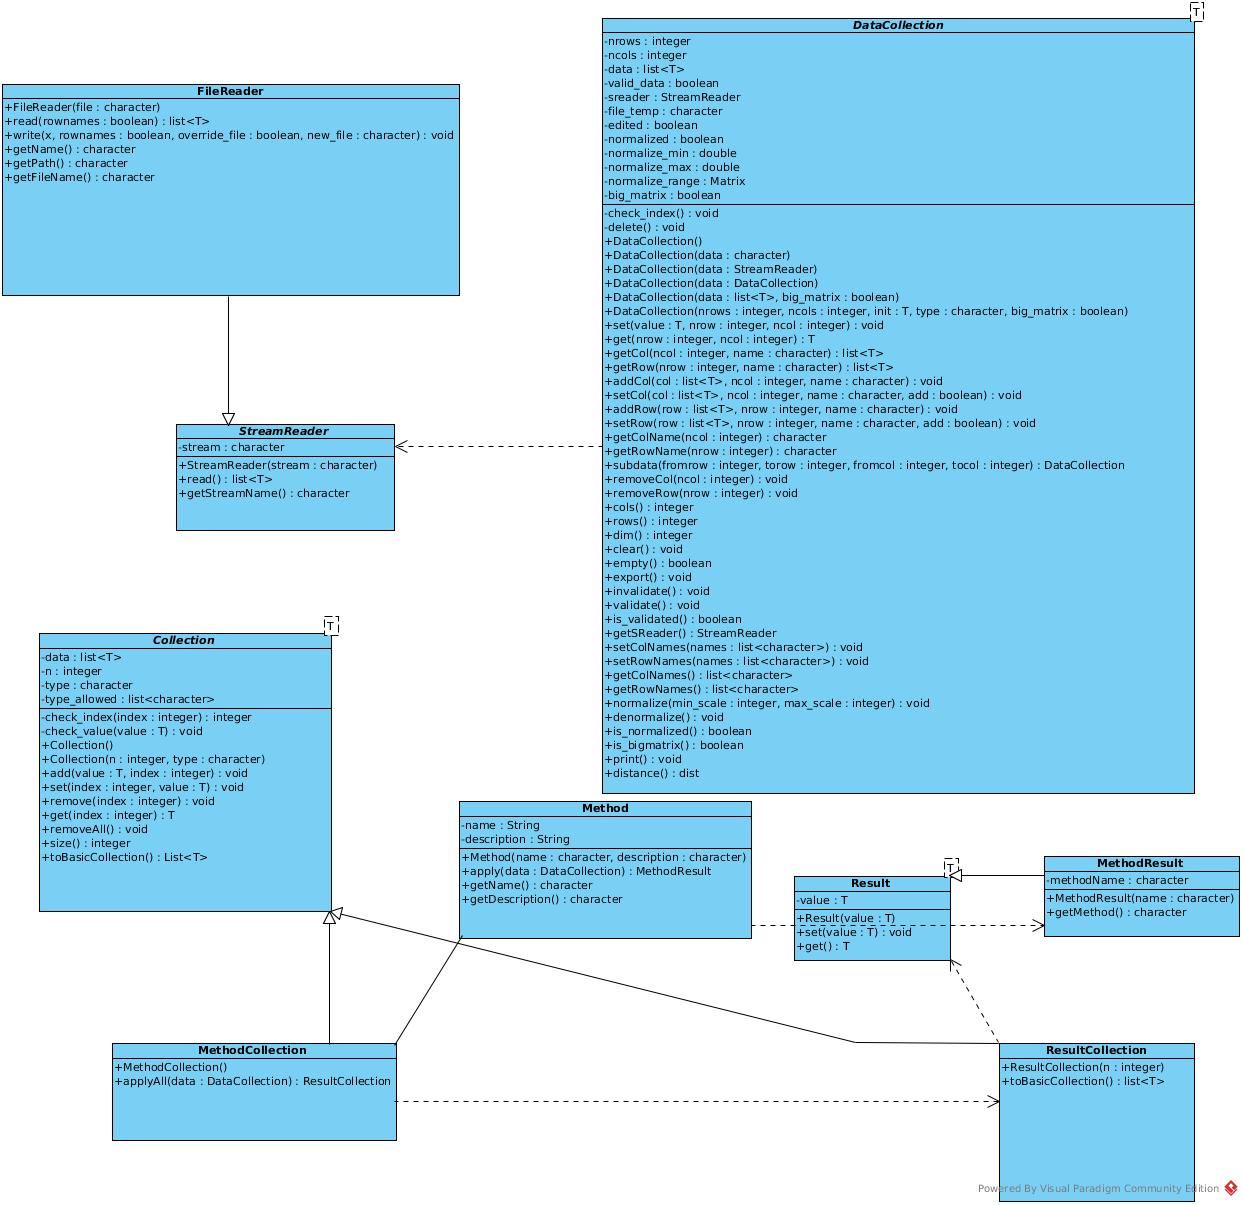
\includegraphics[scale=0.35]{DataUtilsR.jpg}
	\\Imagen 4: Diagrama de clases del paquete R DataUtils.
	\end{center}
\end{landscape}

\begin{landscape}
	\begin{center}
	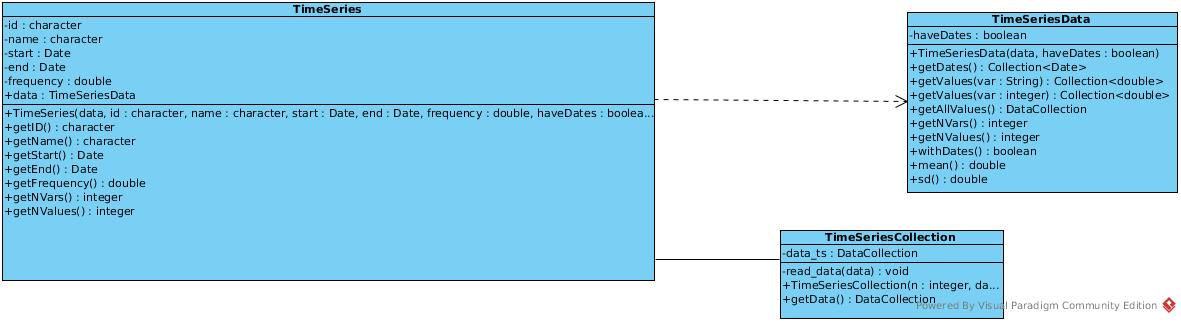
\includegraphics[scale=0.5]{TimeSeriesR.jpg}
	\\Imagen 5: Diagrama de clases del paquete R TimeSeries.
	\end{center}
\end{landscape}

\begin{landscape}
	\begin{center}
	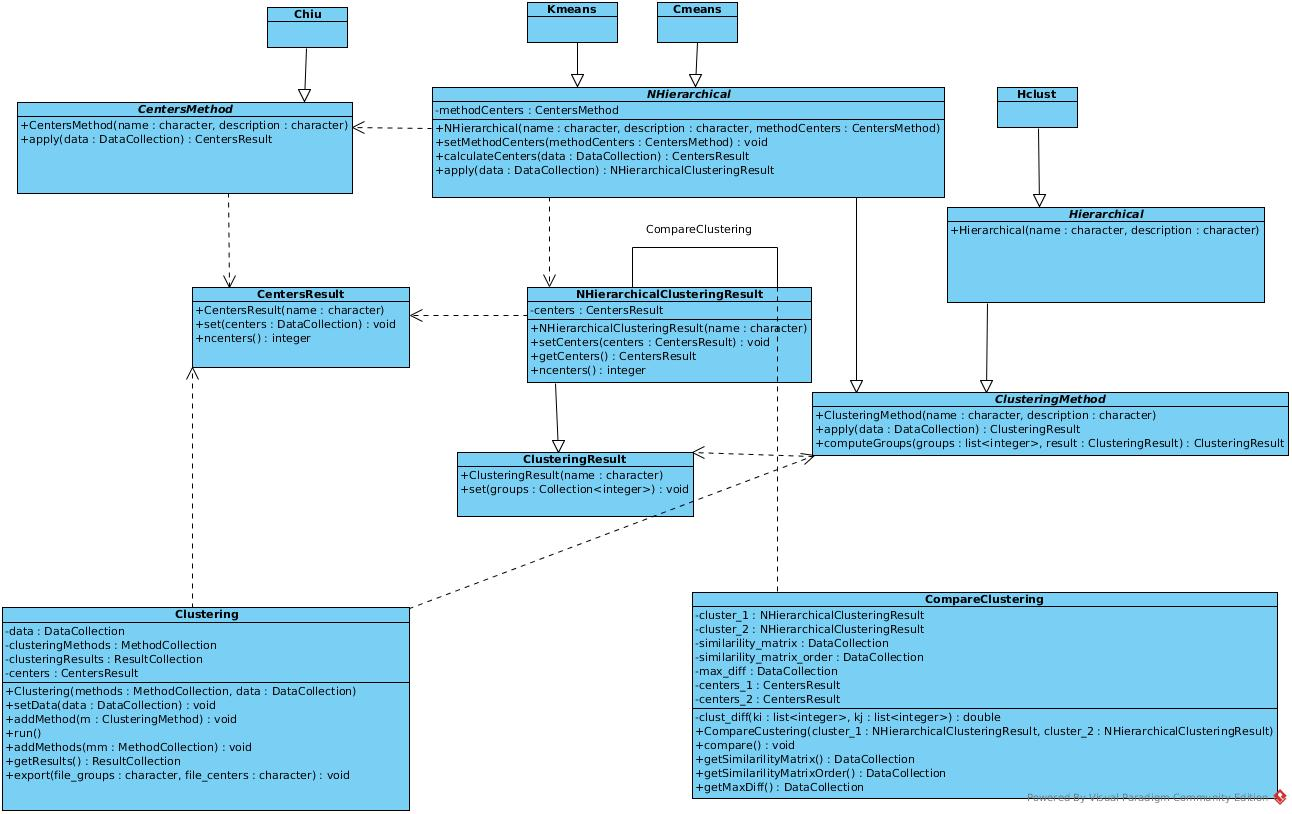
\includegraphics[scale=0.4]{ClusteringR.jpg}
	\\Imagen 6: Diagrama de clases del paquete R Clustering.
	\end{center}
\end{landscape}

\begin{landscape}
	\begin{center}
	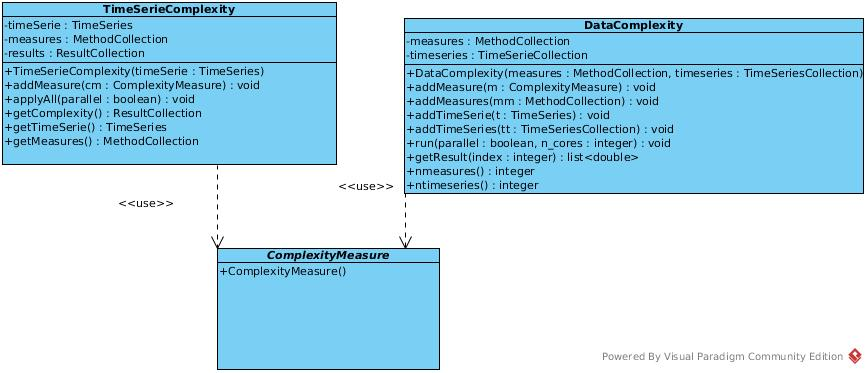
\includegraphics[scale=0.5]{ComplexityR.jpg}
	\\Imagen 7: Diagrama de clases del paquete R TimeSeriesComplexity.
	\end{center}
\end{landscape}

\begin{landscape}
	\begin{center}
		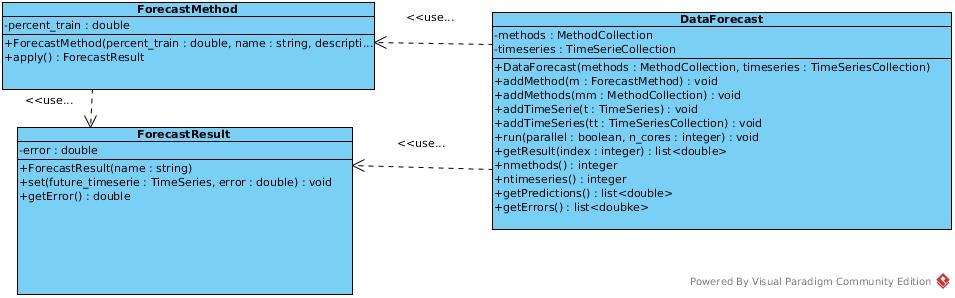
\includegraphics[scale=0.6]{ForecastR.jpg}
		\\Imagen 8: Diagrama de clases del paquete R TimeSeriesForecast.
	\end{center}
	\begin{center}
		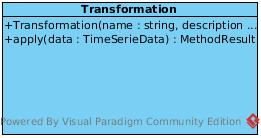
\includegraphics[scale=0.6]{TransformationR.jpg}
		\\Imagen 9: Diagrama de clases del paquete R TimeSeriesTransformation.
	\end{center}
\end{landscape}

\begin{landscape}
	\begin{center}
	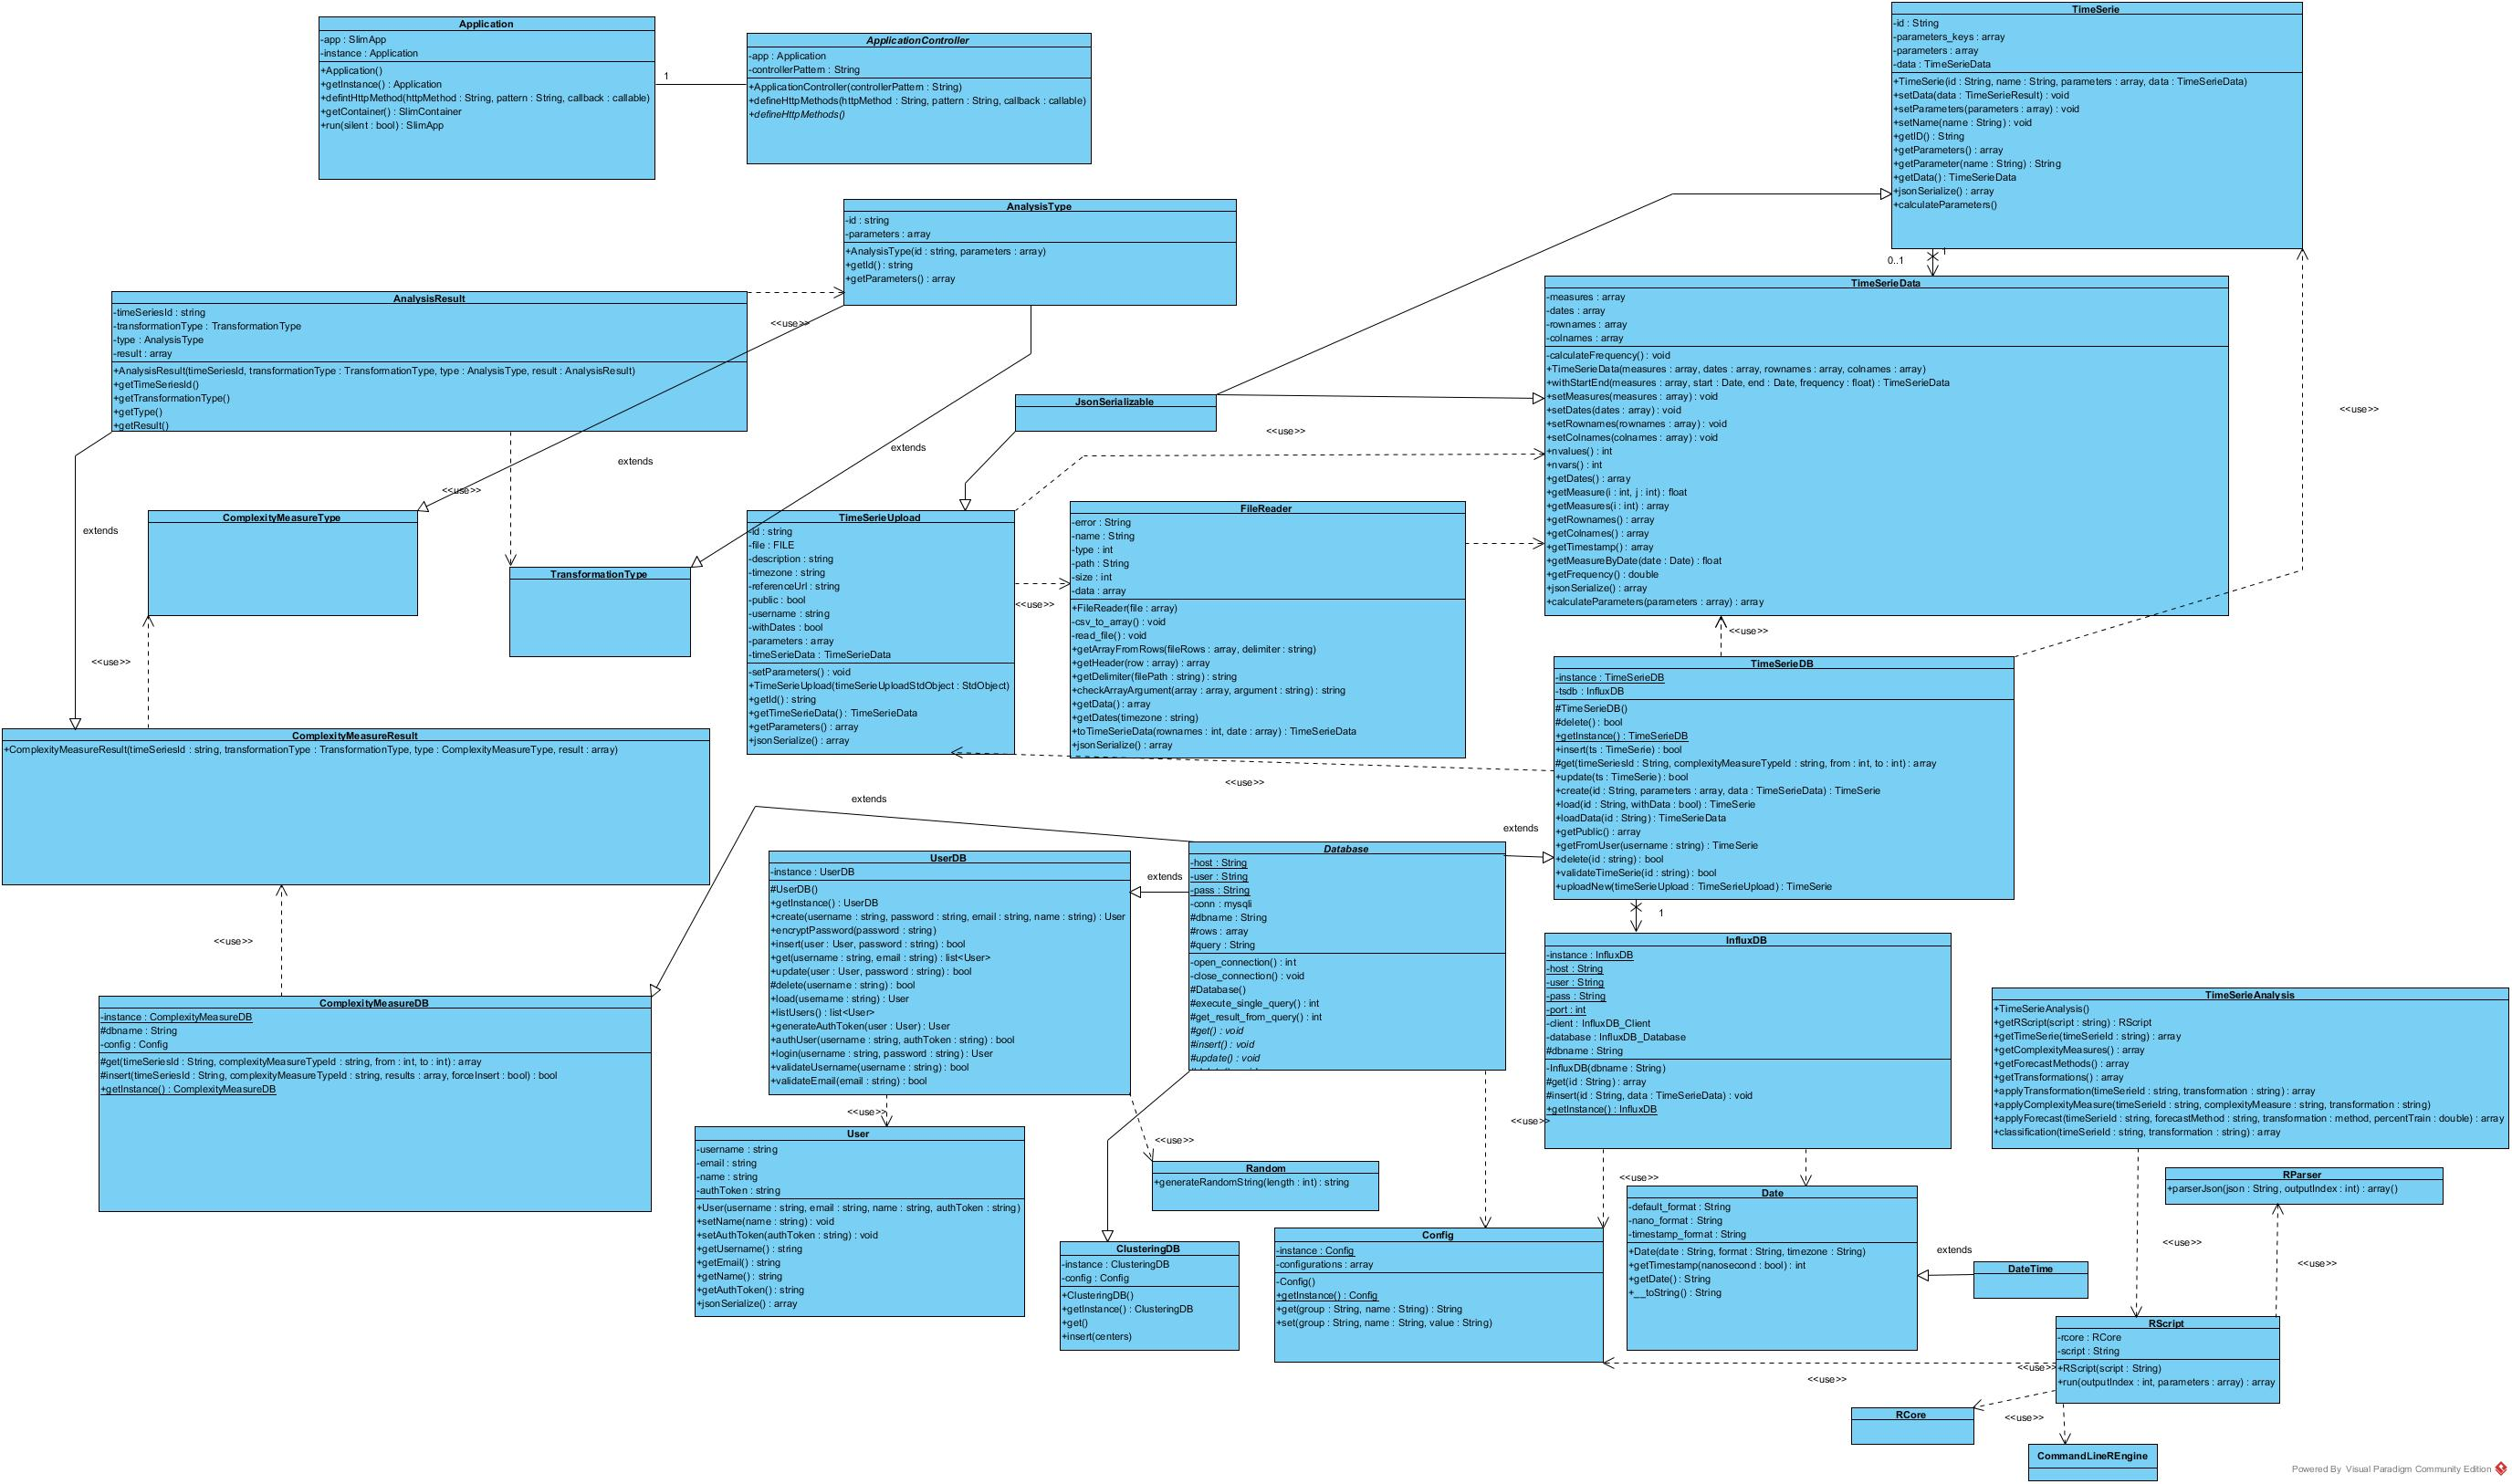
\includegraphics[scale=0.25]{TimeSeriesAnalysisAPI.jpg}
	\\Imagen 10: Diagrama de clases API PHP (TimeSeriesAnalysisAPI)
	\end{center}
\end{landscape}

\begin{landscape}
	\begin{center}
	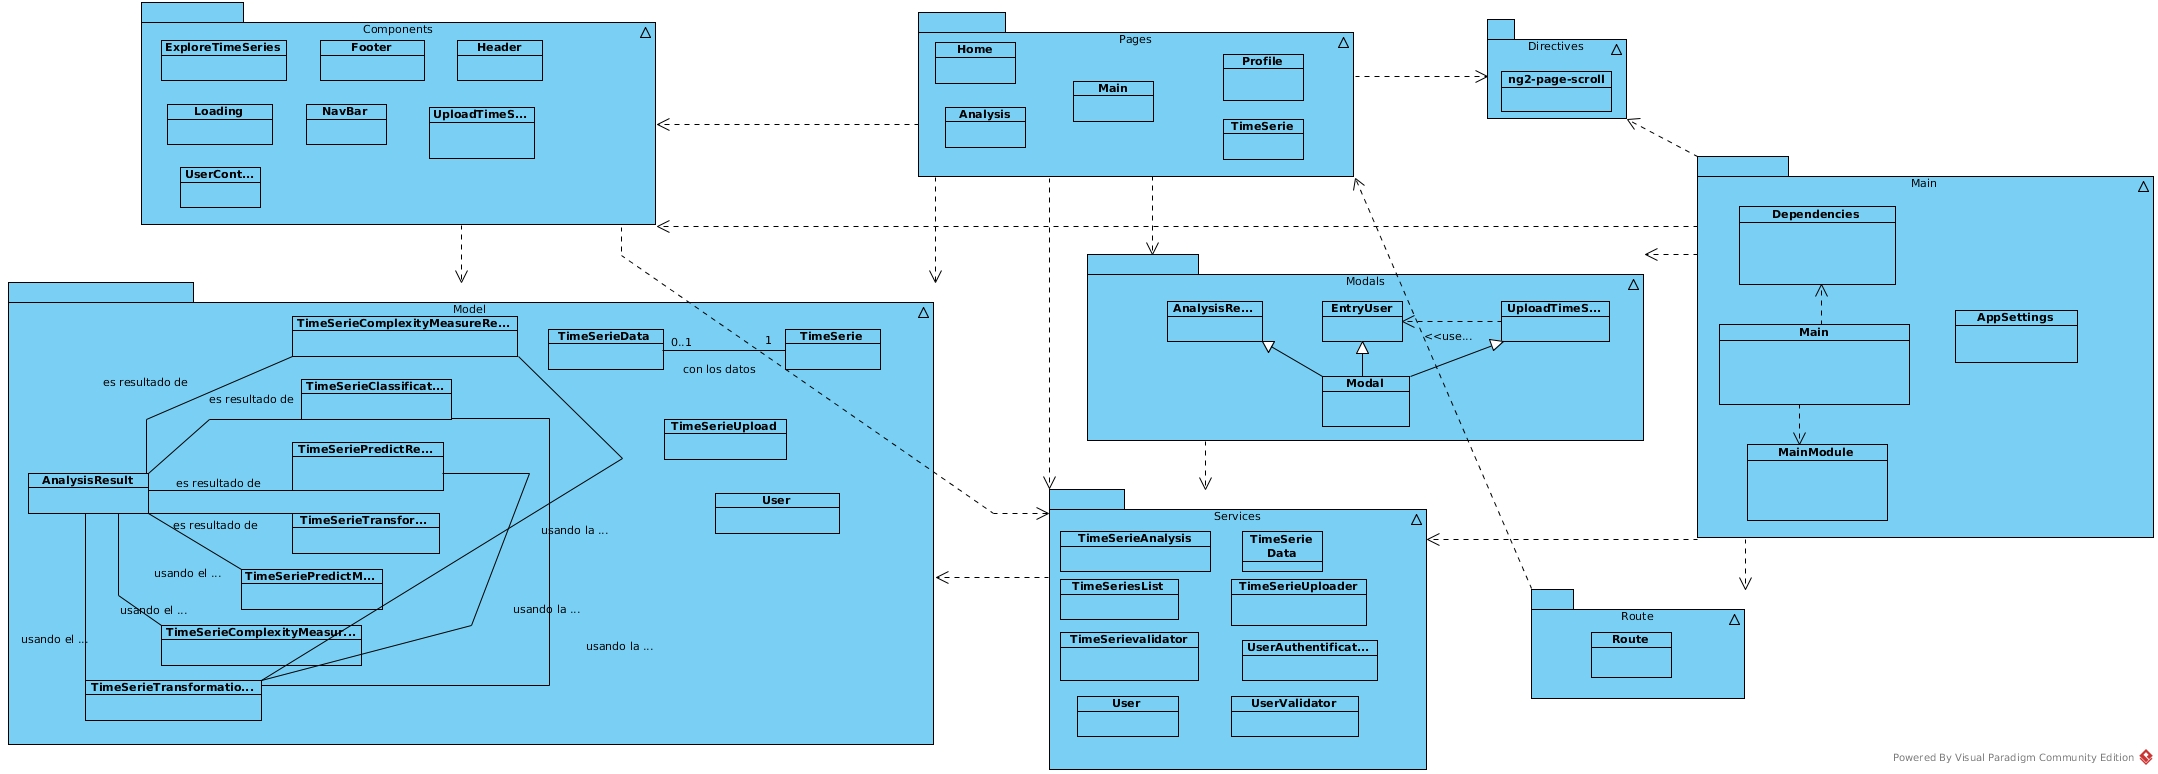
\includegraphics[scale=0.3]{TimeSeriesAnalysisApp.jpg}
	\\Imagen 11: Diagrama de clases Angular Aplicación Web. (TimeSeriesAnalysisApp)
	\end{center}
\end{landscape}

\newpage
\subsection{Interfaces de usuario}\label{sec:interfacesdeusuario}
\begin{center}
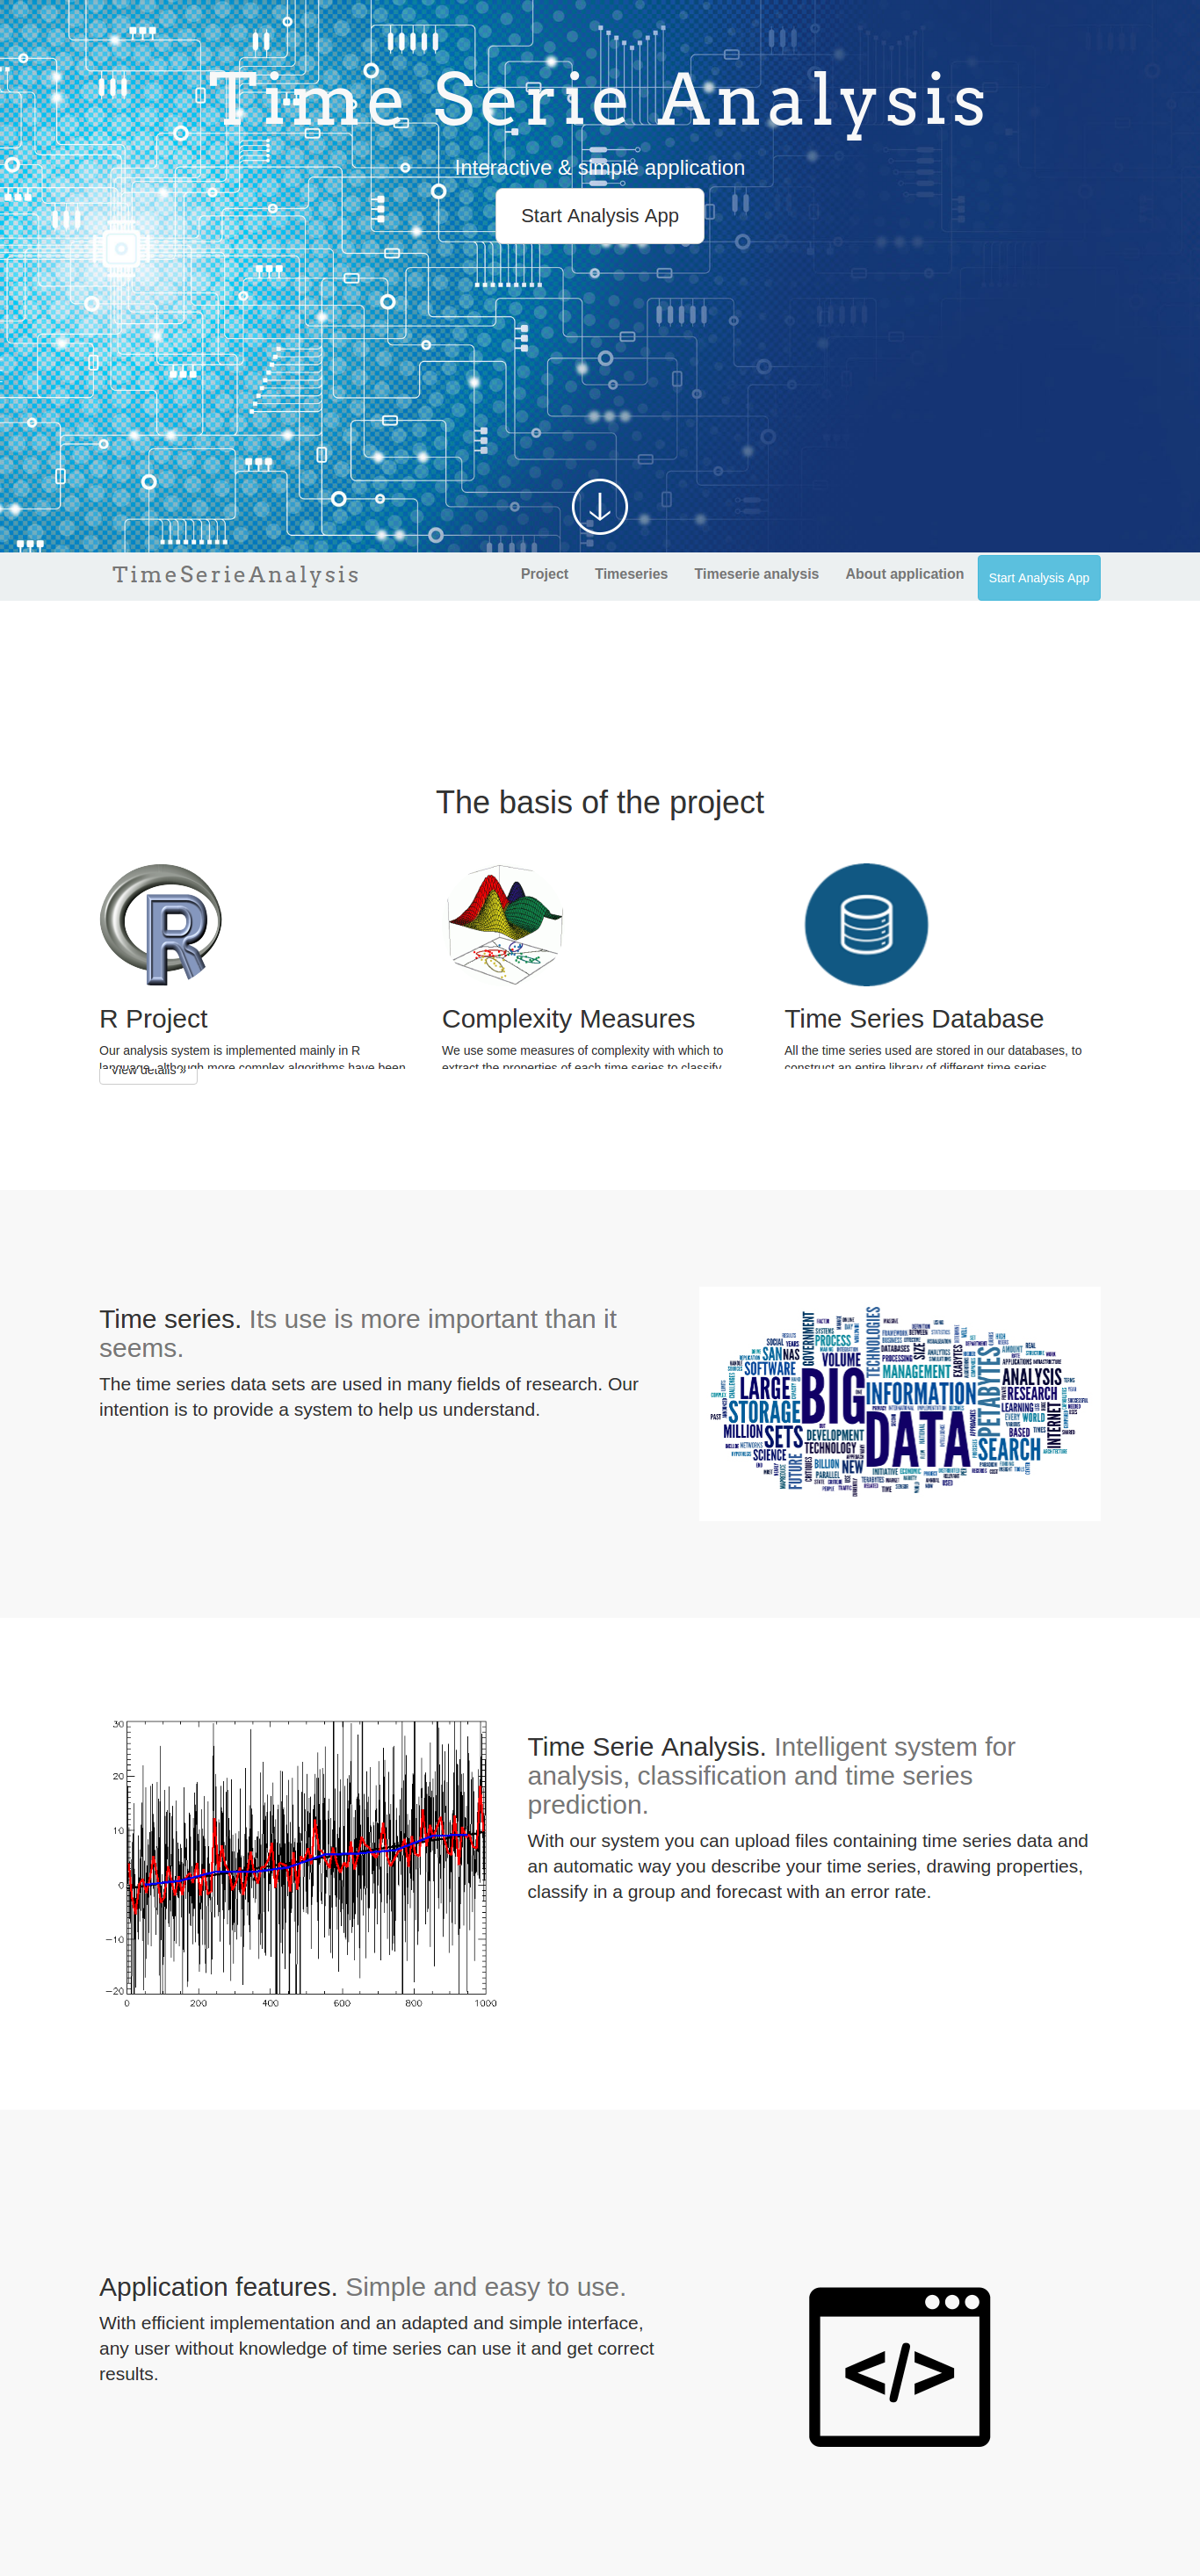
\includegraphics[scale=0.2]{HomePage.png}
\\Imagen 12: Página principal
\end{center}
Desde la página principal se inicia la aplicación con los dos botones superiores (Start Analysis App). Y se mueve por la página seleccionando los diferentes enlaces de la barra de navegación.
\begin{center}
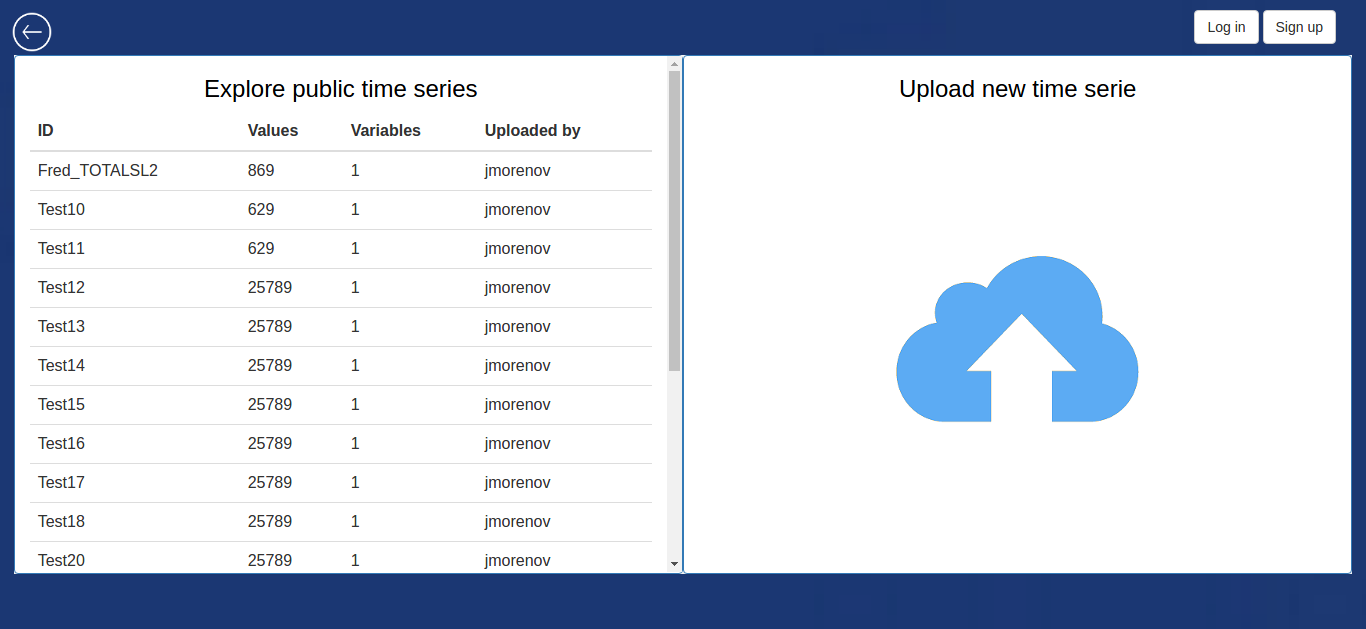
\includegraphics[scale=0.35]{AnalysisPage.png}
\\Imagen 13: Página de inicio de la aplicación.
\end{center}
En esta página se puede iniciar sesión o registrarse desde los dos botones superiores, estos botones abren un modal (Imágenes 14 y 15). A la iquierda está una flecha para volver a la página de inicio y la lista de series temporales públicas, seleccionando cualquiera de ellas se abrirá la página de serie temporal (Imagen 17). Y a la derecha el botón para subir una nueva serie temporal, al hacer click se abrirá otro modal con las diferentes opciones (Imagen 16).

\begin{center}
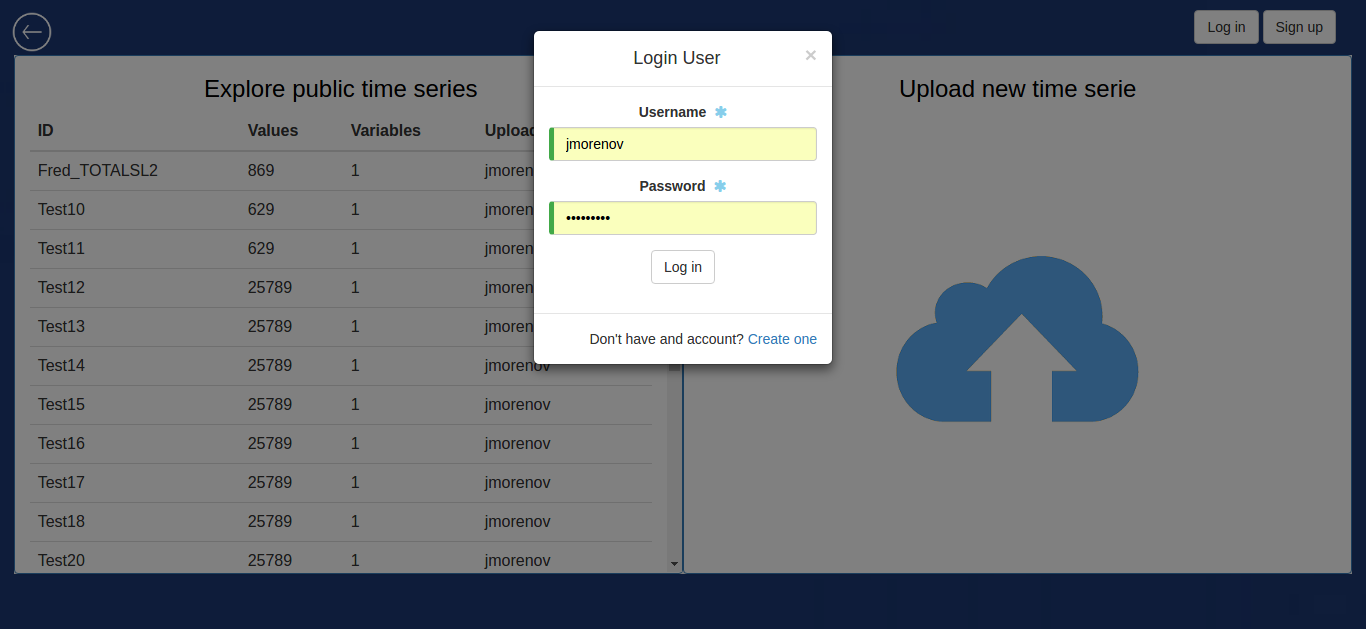
\includegraphics[scale=0.35]{LoginUser.png}
\\Imagen 14: Modal de inicio de sesión.
\end{center}

\begin{center}
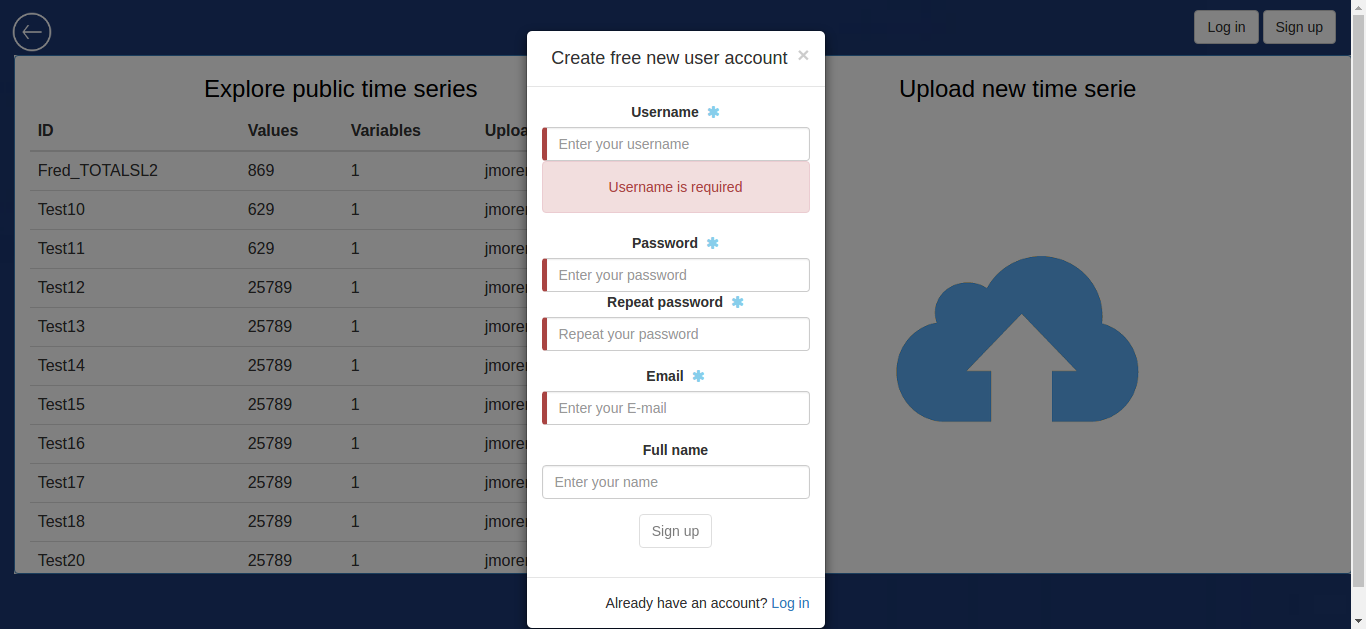
\includegraphics[scale=0.35]{RegisterUser.png}
\\Imagen 15: Modal de registro de usuario.
\end{center}

\begin{center}
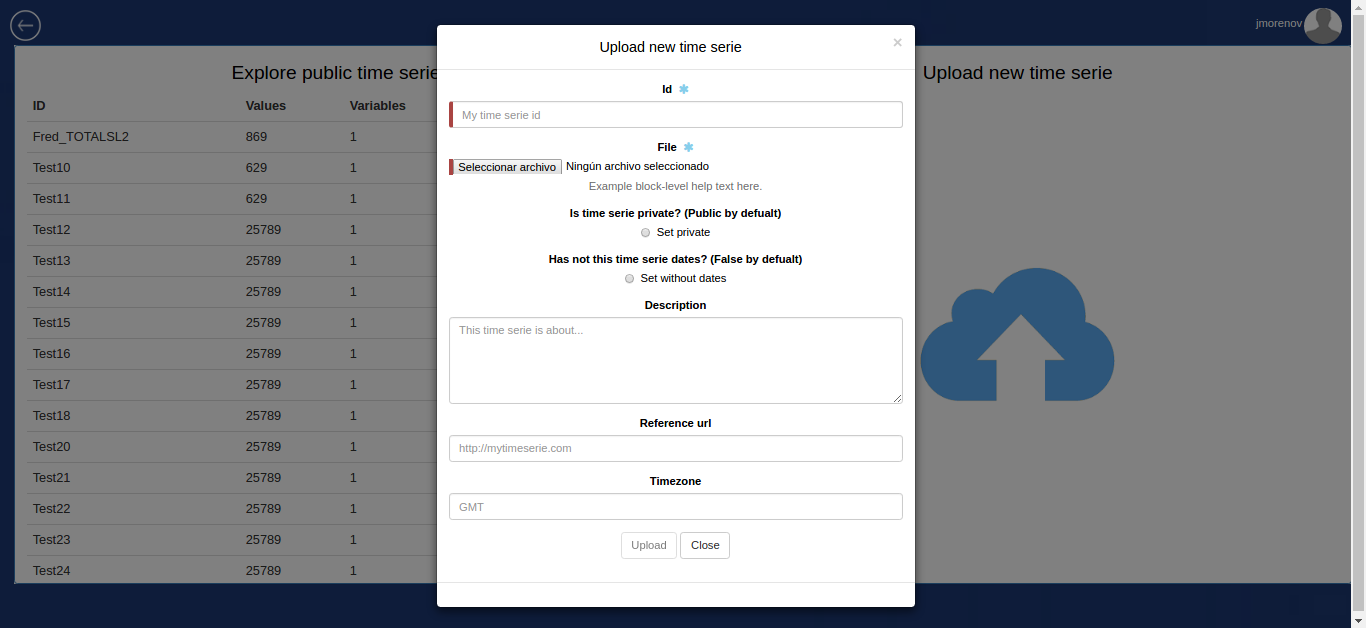
\includegraphics[scale=0.35]{UploadTimeSeries.png}
\\Imagen 16: Modal para subir nueva serie temporal.
\end{center}

\begin{center}
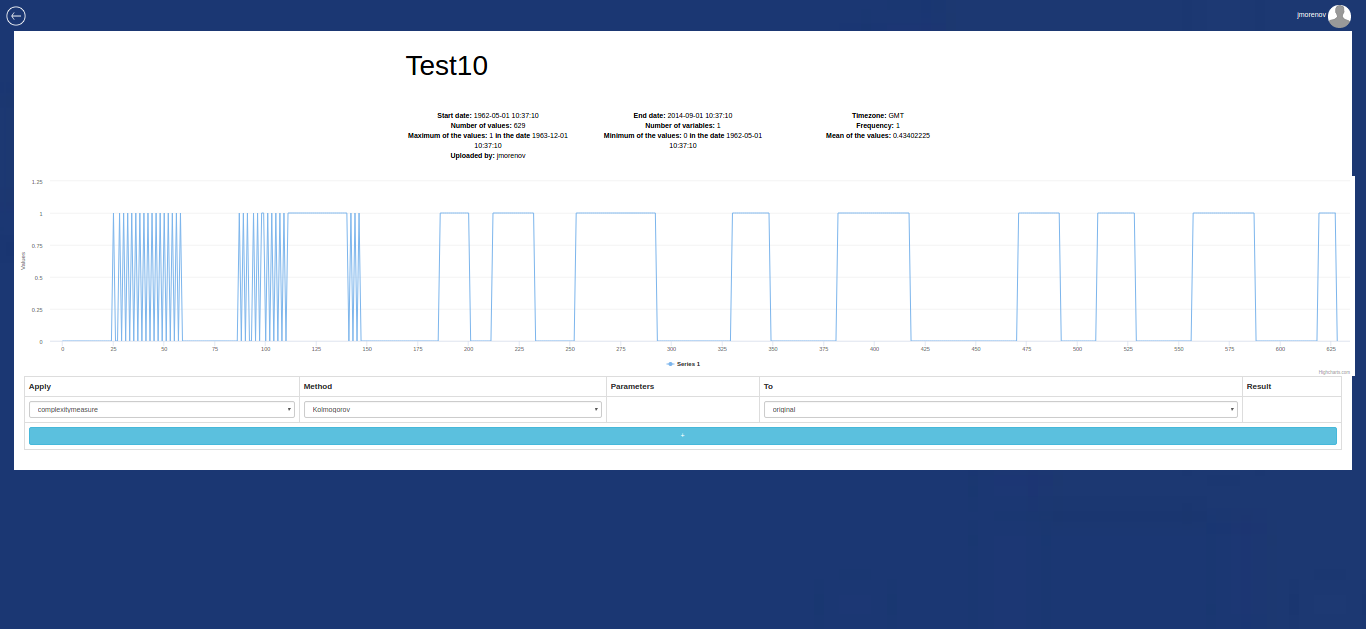
\includegraphics[scale=0.35]{TimeSeriesPage.png}
\\Imagen 17: Página de serie temporal.
\end{center}

En la página de serie temporal nos encontramos con todas las propiedades básicas de la misma, una gráfica con sus datos y la tabla para aplicar análisis al final. Si se hace click en la imagen de usuario en la esquina superior derecha se abrirá un dropdown (Imagen 18).

\begin{center}
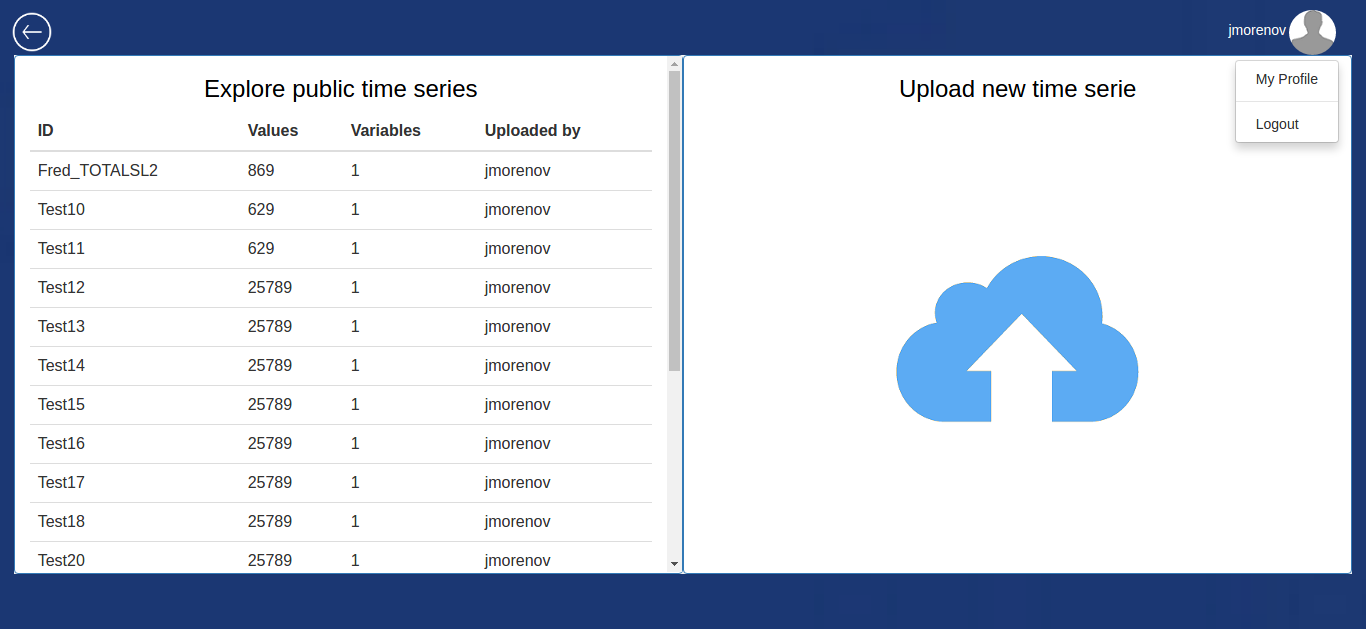
\includegraphics[scale=0.35]{DropdownUser.png}
\\Imagen 18: Dropdown con las opciones de usuario (Usuario logueado).
\end{center}

En este dropdown se puede navegar hacia la página de perfil de usuario (Imagen 19) o cerrar sesión.

\begin{center}
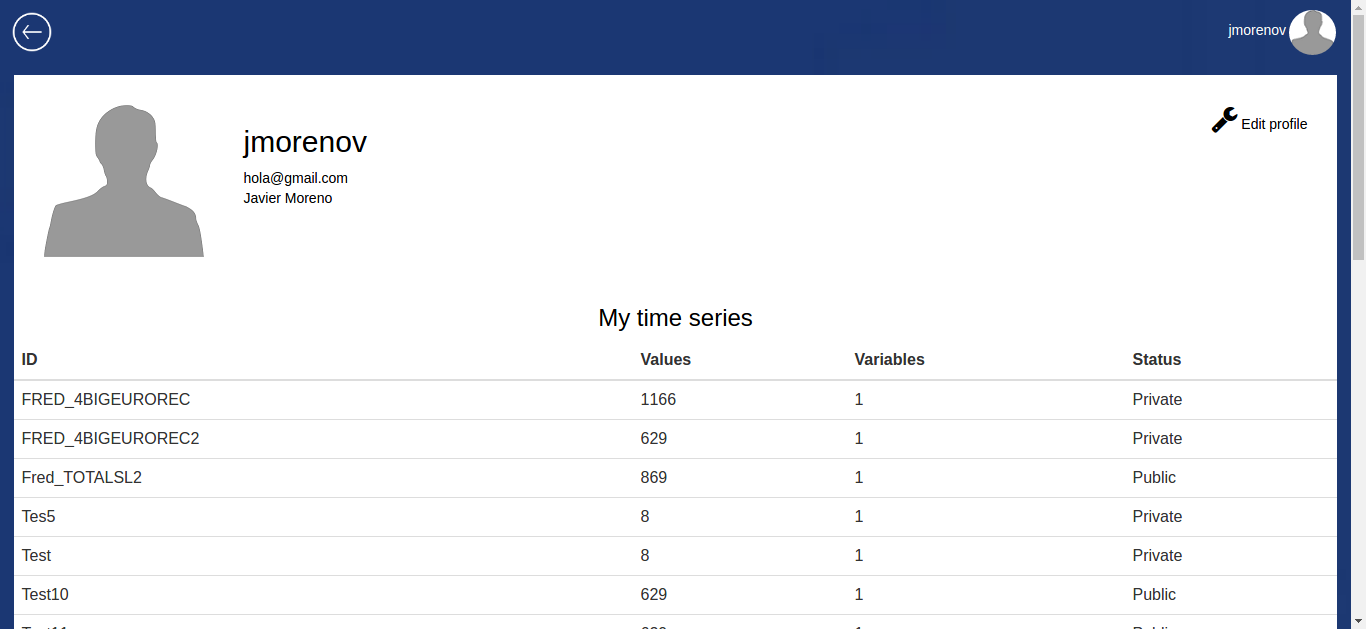
\includegraphics[scale=0.35]{ProfileUserPage.png}
\\Imagen 19: Página de perfil de usuario.
\end{center}
En esta página se muestra el perfil de usuario junto con una lista de sus series temporales, públicas y privadas, si son privadas solo el propio usuario puede acceder a ellas, obteniendo un mensaje de error si accediera un usuario sin permisos. Además tenemos la opción de editar el perfil si se hace click en el elemento de la derecha (Imagen 20).
\begin{center}
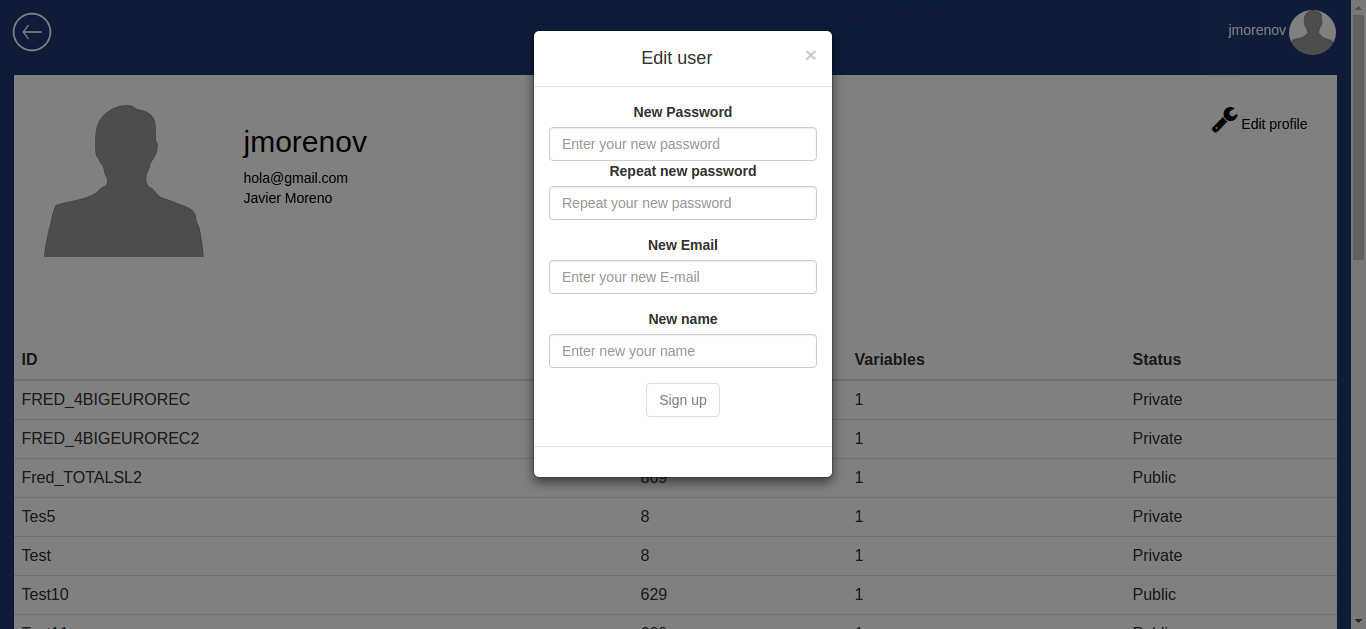
\includegraphics[scale=0.35]{EditUserProfile.png}
\\Imagen 20: Modal de editar perfil de usuario.
\end{center}
\newpage
\subsection{Herramientas utilizadas}
En este desarrollo se han utilizado diversas herramientas de apoyo como bibliotecas externas que nos ofrecen distintas funcionalidades y software de apoyo al desarrollo. Este software usado ha sido:\\\\
\textbf{• Git \citep{wiki:git}:} Software de control de versiones donde se ha ido subiendo el código desarrollado.\\\\
\textbf{• Docker \citep{wiki:docker}:} Software que ofrece contenedores para el despliegue de aplicaciones. Es de gran utilidad para el despliegue en la nube. En este proyecto se han utilizado un total de 10 contenedores Docker y gracias a ellos el sistema completo puede hacerse distribuido muy fácilmente.\\\\
\textbf{• RStudio \citep{wiki:rstudio}:} IDE para el desarrollo en R, que dispone además de un gestor de paquetes.\\\\
\textbf{• Phpstorm \citep{web:phpstorm}:} IDE para el desarrollo en PHP.\\\\
\textbf{• PyCharm \citep{web:pycharm}:} IDE para el desarrollo en Python.\\\\
\textbf{• Youtrack \citep{web:youtrack}:} Aplicación web, montada sobre Docker, para ayudar al desarrollo en Scrum.\\\\
\textbf{• Teamcity \citep{web:teamcity}:} Aplicación web, montada también sobre Docker, que lleva el control del código y la integración continua. Ha sido muy útil para controlar fallos tempranos de compilación de código o ejecucución de tests.\\\\ 
\textbf{• Npm \citep{wiki:npm}:} Gestor de paquetes para Angular.\\\\
\textbf{• Composer \citep{web:composer}:} Gestor de paquetes para PHP.\\\\
\textbf{• Visual paradigm \citep{web:visualparadigm}:} Software para el diseño de diagramas.\\\\
\textbf{• InfluxDB \citep{web:influxdb}:} Este software es una base de datos de series temporales a la cual se accede mediante consultas http. Almacena las series temporales como datos y fechas, pudiendo añadir además Tag y teniendo un identificador único. De no definir fechas al insertar la serie temporal las fechas que se añaden son el timestamp del momento de inserción. Además ofrece bibliotecas muy útiles, en este caso se ha usado una para acceder mediante PHP (influxdb-php \citep{github:influxdb}) con la que se accede desde la API.\\\\
\textbf{• Apache \citep{wiki:apache}:} Software para el desarrollo de servidores web.\\\\
\textbf{• PhpMyAdmin \citep{wiki:phpmyadmin}:} Aplicación web para la gestión de datos en un servidor sql.\\\\
El desarrollo de la biblioteca de análisis, TimeSeriesAnalysisLibrary, ha sido realizado en RStudio y se ha hecho uso de diversos paquetes, siendo los más importantes:
\begin{itemize}
	\item R6 \citep{pdf:r6}: Ofrece el desarrollo orientado a objetos en R.
	\item entropy \citep{pdf:entropy}: Medidas de complejidad de entropía.
	\item parallel \citep{pdf:parallel}: Ejecución en paralelo.
	\item testthat \citep{pdf:testthat}: Métodos para testear código en R.
	\item forecast \citep{pdf:forecast}: Predicción de series temporales.
	\item xts \citep{pdf:xts}: Métodos para interactuar con series temporales.
	\item Rcpp \citep{pdf:rcpp}: Desarrollo de funciones para R en C++.
	\item RcppParallel \citep{web:rcppparallel}: Funciones C++ en paralelo.
	\item bigmemory \citep{pdf:bigmemory}: Genera archivos temporales para trabajar con archivos muy grandes.
\end{itemize}
La API, TimeSeriesAnalysisAPI, se ha desarrollado usando PhpStorm y Composer, y los paquetes utilizados han sido:
\begin{itemize}
	\item guzzle \citep{github:guzzle}: Ofrece funcionalidad para realizar peticiones Http.
	\item influxdb-php \citep{github:influxdb}: Desarrollado para hacer peticiones a una base de datos Influxdb.
	\item slim \citep{web:slim}: Framework para desarrollar una API en Php.
	\item phpunit \citep{web:phpunit}: Framework que ofrece la funcionalidad para ejecutar tests sobre Php.
\end{itemize}
Por último la aplicación web, TimeSeriesAnalysisWebApp, se ha desarrollado con PhpStorm (también ofrece desarrollo web javascript) y usando Npm como gestor de paquetes. Los paquetes más importantes han sido:
\begin{itemize}
	\item angular \citep{web:angular_google}: Framework para el desarrollo web.
	\item bootstrap \citep{web:bootstrap}: Framework que ayuda al desarrollo web ofreciendo gran diversidad de estilos css.
	\item highcharts \citep{web:highcharts}: Ofrece funcionalidad para generar gráficos.
	\item karma \citep{web:karma}: Ofrece funcionalidad para ejecutar tests.
	\item ngx-modal \citep{web:ngx-modal}: Ofrece funcionalidad para mostrar modales.
\end{itemize}

\newpage
\section{Biblioteca de análisis (TimeSeriesAnalysisLibrary)}\label{sec:bibliotecadeanalisis}
La biblioteca de análisis (TimeSeriesAnalysisLibrary) es un conjunto de métodos que ofrecen funcionalidad que se puede aplicar a series temporales, la principal es la de analizar series temporales. La idea es que todo sea lo más transparente al usuario posible, es decir, el usuario seleccionaría un archivo y la biblioteca se encargaría del resto.\\\\La biblioteca ofrece la siguiente funcionalidad para aplicar sobre series temporales:
\begin{itemize}
	\item Medidas de complejidad
	\item Transformaciones
	\item Clustering
	\item Predicción
	\item Clasificación
\end{itemize}
Todos estos métodos de análisis pueden ser aplicados individualmente o en grupos, por ejemplo todas las medidas de complejidad a la vez sobre una o sobre un conjunto de series temporales. Este tipo de cálculos son útiles para el uso de Clustering que será explicado más adelante.\\\\Vamos a analizar uno a uno los métodos generales, o módulos de la biblioteca, empezando por las medidas de complejidad.

\subsection{Medidas de complejidad}\label{sec:medidasdecomplejidad}
Una medida de complejidad es un cálculo que se aplica sobre un conjunto de datos, en este caso series temporales,  y devuelve como resultado la complejidad de los datos de ésta. Estos resultados son una de las partes más importantes de este proyecto ya que se usan para clasificar series temporales respecto a su complejidad, en el Clustering.\\\\
Las medidas de complejidad, que implementa la biblioteca son las siguientes:\\\\
- \textbf{Kolmogorov}\cite{article:kolmogorov}\cite{wiki:kolmogorov}\\
La complejidad Kolmogorov K(x) de un objeto x es la longitud, en bits, de el programa más pequeño (en bits) que puede ejecutarse en una Máquina de Turing Universal \cite{wiki:maquinaturing} (U), devuelve K(x) y finaliza la ejecución. Esta medida fue desarrollada independientemente por Andrey N. Kolmogorov en el final de los años 60.\\
La complejidad Kolmogorov de una serie temporal \(x_{i}\), i=1,2,3,4...,N; puede ser calculada de la siguiente forma \cite{article:kolmogorovcomplexity}: \\\\
\underline{Paso 1:} Codificar la serie temporal construyendo una secuencia s, formada con los caracteres 0 y 1, escrital: s(i), i=1,2,3,4,...,N; según la regla:
$$s(i)= \left\{ 
\begin{array}{lcc}
0 & x_{i} < x_{*} \\
1 & x_{i} \geq x_{*} 
\end{array}
\right.
$$
Donde \(x_{*}\) es un umbral, el valor medio de la serie temporal se usa con frecuencia como el umbral.\\
\underline{Paso 2:} Calcular el contador de complejidad C(N), el cual está definido como el número mínimo de patrones distintos contenidos en una secuencia de caracteres.\\\\
- \textbf{Lempel-Ziv}\cite{article:lempelziv}\\
Esta medida de complejidad está basada en la idea de Kolmogorov, Lempel y Ziv desarrollaron el algoritmo (LZA), el cuál es con frecuencia usado en la evaluación de la aleatoriedad de las secuencias finitas como una medida de su desorden.\\\\Primero se calcula la complejidad de Kolmogorov K(x) de un objeto x y luego la complejidad normalizada \(C_{k}(N)\), la cuál está definida por la ecuación:
\begin{equation}
\label{eq:kolmogorovnormalized}
C_{k}(N) = \frac{c(N)}{b(N)} = c(N)\frac{log_2 N}{N}
\end{equation}
\textbf{- Aproximation Entropy}\\
Aproximation Entropy (ApEn) es una medida de complejidad utilizada para cuantificar la cantidad de regularidad y la imprevisibilidad de las fluctuaciones sobre los datos de series temporales. La presencia de patrones repetitivos de fluctuación en una serie temporal la hace más predecible que una serie temporal en la que tales patrones están ausentes.\\\\ApEn refleja la probabilidad de que patrones de observaciones similares no sean seguidos por otras observaciones similares también. Una serie temporal que contiene muchos patrones repetitivos tiene un ApEn relativamente pequeño, mientras que una menos predecible tiene uno mayor.\\\\
\textbf{- Sample Entropy}\\
Sample entropy (SampEn) es una modificación de approximate entropy, utilizada ampliamente para evaluar la complejidad de una señal temporal fisiológica, diagnosticando así enfermedades. Al igual que ApEn, SampEn es una medida de complejidad pero no incluye patrones auto-similares como hace ApEn.\\\\
\textbf{- Permutation Entropy}\\
Permutation entropy (PE) es una medida de complejidad, para series temporales arbitrarias, basada en el análisis de patrones de permutación.\\\\
Entrada: Dada una serie temporal \(X = \{x_{i}\}_{i=1...N}\)\\
Hay que determinar la longitud de la ventana deslizante n y deslizar la serie temporal de acuerdo a ella, calcular PE \(h_{n}\) de orden n, repetir para varios n y al final calcular \(h_{n}\), donde:
\[H(n) = -\sum p()log p(\pi)\]
\[h_{n} = \frac{H(n)}{(n-1)}\]
\textbf{- Shannon Entropy}\citep{article:shannonentropy}\citep{wiki:shannonentropy}\\Definimos el tamaño de información \(H_{0}(A)\) de un conjunto A como el número de bits necesarios para codificar cada elemento de A independientemente.
\[H_{0}(A) = \log_{2}|A|\]
Basada en esta idea nace Shannon Entropy (ShEn), llamada así por Claude Elwood Shannon \citep{wiki:shannon}, aunque su origen recae en Pauile y von Neumann.\\\\La entropía de A es:
\[H(A) = -\sum_{i=1}^np_{i}\log_{2}p_{i}\]
Donde $p_{i}$ es la probabilidad de que el carácter i aparezca en la secuencia.\\\\
\textbf{- ChaoShen Entropy}\citep{web:chaoshenentropy}\citep{article:entropypackage}\\
Medida de complejidad que calcula ShEn H de la variable aleatoria Y de las muestras observadas y, usando el método de Chao and Shen (2003).\\\\ El estimador de entropía Chao-Shen es un estimador Horvitz-Thompson (1952) aplicado al problema de la estimación de entropía, con una corrección de cobertura adicional según lo propuesto por Good (1953).\\\\
\textbf{- Dirichlet Entropy}\citep{web:dirichletentropy}\\
El estimador de entropía de Dirichlet es un estimador bayesiano de plug-in: en la definición de la entropía de Shannon las probabilidades de bin son reemplazadas por las respectivas estimaciones bayesianas de las frecuencias, usando un modelo con una probabilidad Dirichlet anterior y multinomial.\\\\
\textbf{- MillerMadow Entropy}\citep{web:millermadowentropy}\citep{web:millermadowentropyr}\\\\
Esta medida de complejidad estima la entropía de Shannon H de la variable aleatoria Y de las muestras observadas y, aplicando la corrección Miller-Madow a la entropía empírica.\\\\
En 1955 George Miller propuso una simple corrección al estimador naive plugin $\hat{H}_N$ añadiendo el desplazamiento constante en la expresión de sesgo:
\[\hat{H}_M=\hat{H}_N+\frac{K-1}{2n}\]
Esto es una mejora sobre el estimador plugin, pero el desplazamiento añadido no depende de la distribución, sino sólo del tamaño de la muestra. Una variante mejora esta corrección, actua sobre el caso del alfabeto infinito y es llamada: estimador Miller-Madow. En él la cantidad K es estimada desde los datos.\\\\
\textbf{- Shrink Entropy}\citep{web:shrinkentropy}\\\\
Shrink Entropy es una medida de complejidad basada en el estimador shrinkage que es un estimador James-Stein. Es en esencia un estimador dirichlet, donde pseudocount es estimada desde los datos.

\subsection{Transformaciones}\label{sec:transformaciones}
En la biblioteca están incluidas varias transformaciones sobre datos. A continuación se muestran estas transformaciones con sus fórmulas respectivas. Sea X una serie temporal:\\\\
\textbf{- Transformación Cúbica}\\
\[TransCub(X) = X^3\]
\textbf{- Transformación Logarítmica Natural}\\
\[TransLN(X) = log(X)\]
\textbf{- Transformación Logarítmica Base 10}\\
\[TransL10(X) = log_{10}(X)\]
\textbf{- Transformación Logarítmica Base 2}\\
\[TransL2(X) = log_{2}(X)\]
\textbf{- Transformación Exponencial}\\
\[TransExp(X) = exp(X)\]
\textbf{- Transformación Raiz Cuadrada}\\
\[TransSqrt(X) = sqrt(X)\]
\textbf{- Transformación Valor Absoluto}\\
\[TransAbs(X) = abs(X)\]
\textbf{- Transformación Seno}\\
\[TransSin(X) = sin(X)\]
\textbf{- Transformación Arco Seno}\\
\[TransASin(X) = asin(X)\]
\textbf{- Transformación Coseno}\\
\[TransCos(X) = cos(X)\]
\textbf{- Transformación Arco Coseno}\\
\[TransACos(X) = acos(X)\]
Son transformaciones básicas pero muy útiles para ver como se comportan determinadas series temporales.

\subsection{Clustering}\label{sec:clustering}
Una definición básica de Clustering de datos es: Un algoritmo de agrupamiento (en inglés, clustering) es un procedimiento de agrupación de una serie de vectores de acuerdo con un criterio. Esos criterios son por lo general distancia o similitud. \citep{wiki:clustering}. En general es encontrar subconjuntos de datos, dentro de un conjunto, que sean similares entre sí. En este caso para poder aplicar determinados métodos de análisis de series temporales a un subconjunto y otros a otro, consiguiendo unos mejores resultados.\\\\
TimeSeriesAnalysisLibrary también implementa métodos de clustering, y funcionalidad útil sobre clustering como el cálculo de centros con el método de Chiu. Esta basado en el cálculo de potenciales, si tenemos un conjunto de datos Mxm, $x_i(i=1,...,m)$, se calcula el potencial para cada dato y secuencialmente se selecciona el dato restante de mayor potencial. Se define el potencial del dato $x_i$:
\[P_i=\sum_{j=1}^{M}exp\left(-\frac{4||x_i-x_j||^{2}}{r_a^{2}}\right)\] 
Siendo $||x_i-x_j||$ la distancia Euclidea entra $x_i$ y $x_j$, y $r_a$ es un parámetro positivo que controla el decrecimiento del radio del potencial. Este algoritmo está en: \cite[Chapter~6.1.1]{abe2012neural}\\\\
El tipo de clustering se divide en dos: jerárquico y no-jerárquico o de particionamiento. El clustering Jerárquico es un método de análisis de grupos puntuales, el cual busca construir una jerarquía de grupos, básicamente genera un árbol de decisión sobre los datos \citep{wiki:clusteringjerarquico}. El clustering no-jerárquico, a partir de unos centros dados (método de Chiu), genera particiones del conjunto de datos.\\\\La biblioteca implementa métodos de los dos tipos, en primer lugar los jerárquicos son:\\\\
\textbf{- MClust \citep{web:mclustclustering}:} Está dentro del tipo de los jerárquicos pero pertenece a un subconjunto denominado clustering basado en modelos en donde los datos se considera que vienen de una distribución que es la mezcla de dos o más componentes (clusters). Cada componente k (cluster) está modelado por la normal o la distribución Gaussiana la cuál está caracterizada por los parámetros: $\mu_k$ vector medio, $\sum_k$ matriz de covarianza, y una probabilidad asociada al componente, cada punto tiene una probabilidad de pertenecer a cada cluster.\\\\
\textbf{- HClust \citep{web:hclustclustering}:} Este tipo de clustering es por definición jerárquico, pero en esta librería podría ser considerado de particionamiento debido a que aunque se usa su algoritmo principal para generar el árbol de decisión este árbol es podado usando el número de centros de clustering k, que es la base de los clustering de particionamiento.\\\\El algoritmo funciona de la siguiente forma: Selecciona cada punto y lo pone en un cluster propio, selecciona los dos clusters más cercanos y los combina en uno; repite este proceso hasta que todos los puntos (los más cercanos) estén en un mismo cluster.\\\\
Y los no-jerárquicos:\\\\
\textbf{- Fuzzy c-means \citep{wiki:fuzzyclustering}:} Los algoritmos Fuzzy c-Means son algunos de los principales algoritmos utilizados en el agrupamiento difuso y pertenecen a una clase de algoritmos basados en funciones objetivo. Estos algoritmos definen un criterio de agrupamiento en la forma de una función objetivo que depende de la partición difusa. El procedimiento, en sentido general, consiste en minimizar iterativamente esta función hasta obtener una partición difusa óptima.\\\\
\textbf{- K-means \citep{wiki:kmeans}:} Probablemente el algoritmo de agrupamiento más conocido. Tiene como objetivo la partición de un conjunto de n observaciones en k grupos en el que cada observación pertenece al grupo cuyo valor medio es más cercano.

\subsection{Predicción}\label{sec:Prediccion}
La predicción de series temporales es de las partes de más importancia de este trabajo. La biblioteca cuenta con varios métodos de predicción:\\\\
\textbf{- ARIMA \citep{wiki:arima}:} Probablemente el método de predicción de series temporales más conocido. Modelo autorregresivo integrado de promedio móvil (del inglés ARIMA), es un modelo estadístico que utiliza variaciones y regresiones de datos estadísticos con el fin de encontrar patrones para una predicción hacia el futuro. Se trata de un modelo dinámico de series temporales, es decir, las estimaciones futuras vienen explicadas por los datos del pasado y no por variables independientes. Fue desarrollado a finales de los sesenta del siglo XX. Box y Jenkins (1976) lo sistematizaron.\\\\
\textbf{- Ets:} Es un modelo de espacio de suavizamiento exponencial. Basado en la clasificación de métodos como describe Hyndman (2008).\\\\
\textbf{- Holtwinters \citep{wiki:holtwinters}:} El modelo Holt-Winters incorpora un conjunto de procedimientos que conforman el núcleo de la familia de series temporales de suavizamiento exponencial. A diferencia de muchas otras técnicas, el modelo Holt-Winters puede adaptarse fácilmente a cambios y tendencias, así como a patrones estacionales. En comparación con otras técnicas, como ARIMA, el tiempo necesario para calcular el pronóstico es considerablemente más rápido.\\\\
\textbf{- StructTS \citep{web:structts}:} Este método de preducción está basado en los modelos estructurales de series temporales. La idea básica de los modelos de series temporales estructurales es que se establecen como modelos de regresión en los que las variables explicativas son funciones del tiempo con coeficientes que cambian con el tiempo. Así, dentro de un marco de regresión, una tendencia simple sería modelada en términos de una constante y un tiempo con una perturbación aleatoria agregada. Este modelo es fácil de estimar usando mínimos cuadrados ordinarios, pero sufre la desventaja de que la tendencia es determinista.\\\\
\textbf{- Bats \citep{article:bats}:} Método de predicción basado en el modelo BATS, esto es un acrónimo de: Box-Cox transform, Arma errors, Trend and seasonal. Es un modelo que agrupa varios.\\\\
\textbf{- Stl \citep{web:stl}:} Este método de predicción consiste en aplicar un método de predicción no estacional a los datos desestacionalizados y re-estacionalizarlos utilizando el último año del componente estacional.

\subsection{Clasificación}\label{sec:Clasificacion}
Esta es la parte más importante de todo el trabajo, y depende de los métodos explicados en los apartados anteriores para realizar los cálculos necesarios. El resultado que se quería obtener era una clasificación de series temporales, es decir, definir un conjunto finito de etiquetas que asignar a cualquier serie temporal que se requiriera. Con esto se conseguía generar conjuntos de series temporales con propiedades similares y que por lo tanto tendrían resultados parecidos cuando se les aplicaran métodos de predicción, o de cualquier tipo.\\\\Para conseguir esta clasificación se usaron conjuntos grandes de series temporales (200000), a las que se les aplicaría todas las medidas de complejidad explicadas anteriormente.\\\\Con esto tenemos una matriz de resultados y entonces es el momento de aplicar los métodos de clustering, que nos particionaran las series temporales, generando una clasificación previa. A partir de esta clasificación, una por cada método de clustering, faltaba por decidir que método de predicción genera mejores resultados para cada conjunto de series temporales. Este resultado final lo obtenemos aplicando todos los métodos de predicción a cada conjunto de series temporales y calculando el porcentaje medio de éxito método/partición de datos. Y con esto tendremos el método de mejor resultado para cada tipo de serie temporal.\\\\Para clasificar una serie temporal se generan sus medidas de complejidad y se calcula la distancia a los centros, seleccionando la menor distancia; teniendo el centro al que pertenece obtenemos el mejor método de predicción.

\newpage
\section{Implementación}\label{sec:implementacion}
En esta sección se explicará la implementación de código que se ha realizado, mostrándola más detalladamente en las secciones de a continuación.
\subsection{Despliegue en Cloud (DockersProject)}\label{sec:dockersproject}
Con el fin de conseguir una aplicación distribuida en Cloud se ha usado el software Docker \citep{wiki:docker}. Este software nos permite construir contenedores que funcionan como servidores dentro de un servidor padre, se pueden configurar de cualquier forma y hay bastantes contenedores ya construidos por terceros y modificables.\\\\Además para poder iniciar, reiniciar, parar o configurar cualquier contenedor de los que se han construido se hicieron scripts y para hacer estos scripts más reutilizables se ha desarrollado un pequeño proyecto llamado DockersProject.\\\\DockersProject está escrito en python y se gestiona mediante comandos y sus argumentos son los argumentos del comando de ejecución, usa como archivo de configuración de los contenedores un archivo json con todo lo necesario: nombre, imagen, localización de la imagen, variables de entrada, puertos, etc. Este archivo se puede modificar facilmente para añadir más contenedores o modificar los existentes y el comando es muy sencillo, por ejemplo: python DockersControl.py --start-all, este comando lanzaría todos los contenedores.\\\\Los contenedores que se han usado han sido:
\begin{itemize}
	\item TimeSeriesAnalysisWebApp: Este contenedor tiene instalado NPM \citep{wiki:npm} con todos los paquetes javascript necesarios para lanzar la aplicación web, así como scripts para actualizar el código y tener siempre el contenedor con la última versión de la aplicación. Además incluye una versión de Apache.
	\item TimeSeriesAnalysisAPI: Este contenedor tiene instalado composer \citep{web:composer} con los paquetes Php necesarios, así como los scripts para actualizar el código como en el contenedor anterior. También Apache \citep{wiki:apache}, Php y TimeSeriesAnalysisLibrary con todos los paquetes R y los scripts de análisis.
	\item Mysql: Contenedor con un servidor mysql, incluye los scripts sql necesarios para el sistema.
	\item Phpmyadmin: Contenedor con una versión de Phpmyadmin \citep{wiki:phpmyadmin} para acceder a los datos del servidor Mysql fácilmente.
	\item InfluxDB: Contenedor que contiene una versión de InfluxDB \citep{web:influxdb} con todas las series temporales almacenadas en el sistema.
	\item Teamcity: Contenedor con una versión de Teamcity \citep{web:teamcity}.
	\item Youtrack: Contenedor con una versión de Youtrack \citep{web:youtrack}.
	\item TeamcityAgent 1, 2 y 3: Contenedores con un agente de Teamcity cada uno, son usados para ejecutar el código sobre la aplicación Teamcity.
\end{itemize}

\begin{center}
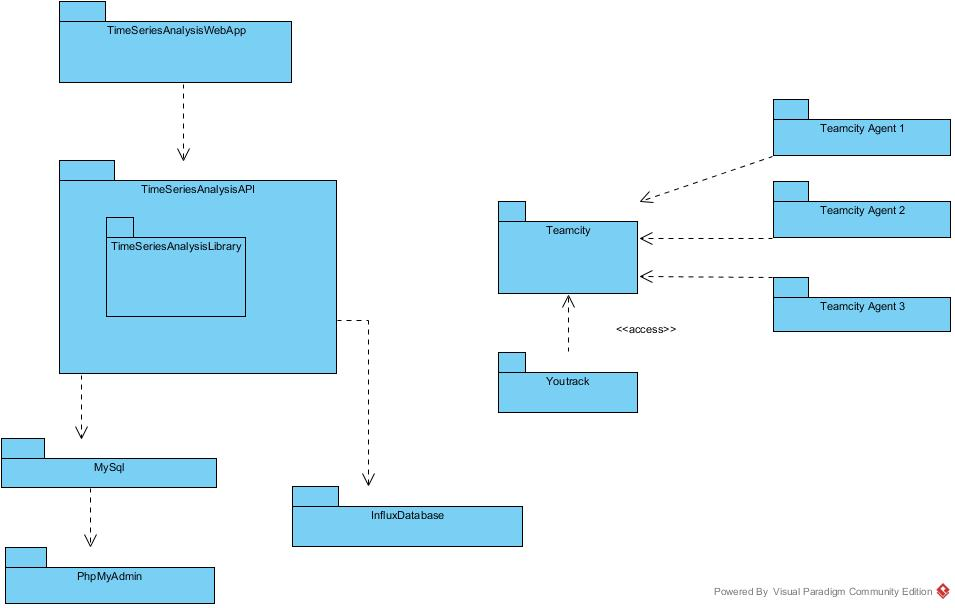
\includegraphics[scale=0.55]{DockerContainers.jpg}
\\Imagen 21: Diagrama de contenedores Docker.
\end{center}

\subsection{Biblioteca de análisis en R (TimeSeriesAnalysisLibrary)}\label{sec:bibliotecar}
La biblioteca de análisis desarrollada en R y C++ es el módulo básico para el análisis de series temporales, todo cálculo que se hace con la serie temporal se ejecuta en la biblioteca obteniendo un resultado.\\\\
La biblioteca ha sido desarrollada siguiendo la programación orientada a objetos. El desarrollo inicio con las clases para poder gestionar series temporales, cargándolas desde archivos, pudiendo exportarlas, y hacer cálculos sobre ellas. Se han diseñado "clases contenedoras" como TimeSeries, TimeSeriesData o para colecciones de datos "Helpers" para hacer cálculos más simples. Todo esto haciendo uso de un gestor de excepciones para mostrar cualquier tipo de error al usuario. Además se crearon clases abstractas sobre las que se crearían las clases finales, ejemplos de esto son las clases Method, Result o Collection. Todas estas clases se pueden ver en el diagrama mostrado anteriormente.\\\\
Debido a problemas de eficiencia en algunos casos, por ejemplo el cálculo del número de centros con el método Chiu, se tuvieron que desarrollar algunas funciones en C++, y el cambio fue muy notable; en algunos casos se pasó de horas a segundos.\\\\Todas las clases desarrolladas en R han sido testeadas para evitar fallos en modificaciones posteriores. Esto se hizo debido a que esta biblioteca es la base de todo el sistema superior y debía funcionar sin problemas.\\\\Estas clases pertenecen a diversos paquetes que se han desarrollado y que se explicaran a continuación, y todos los paquetes juntos forman la biblioteca de análisis TimeSeriesAnalysisLibrary, la cuál ha sido instalada en el servidor junto a todos los paquetes de los que depende. Y se accede mediante scripts escritos en R que son los que llaman los archivos en PHP pertenecientes a la API.\\\\Los paquetes R desarrollados han sido los siguientes:
\begin{itemize}
	\item RLog: Ofrece funcionalidad para gestionar logs de la aplicación y algunas excepciones.
	\item DataUtils: Clases para trabajar con colecciones de datos de cualquier tipo, además de colecciones de un tamaño muy grande y que son necesarias de almacenar en disco.
	\item Clustering: Clases para ejecutar métodos de Clustering sobre conjuntos de datos.
	\item TimeSeries: Clases para trabajar con series temporales.
	\item TimeSeriesComplexity: Métodos para calcular medidas de complejidad a series temporales.
	\item TimeSeriesForecast: Métodos para aplicar métodos de predicción a series temporales.
	\item TimeSeriesTransformation: Métodos para aplicar métodos de transformación a series temporales.
	\item TimeSeriesDatabase: Clases para acceder a TimeSeriesAnalysisAPI.
	\item TimeSeriesAnalysis: Paquete formado por los paquetes anteriores y que contiene scripts para ejecutar análisis de series temporales.
\end{itemize}

Este módulo es el sistema de clasificación, se usa mediante scripts R que se han desarrollado. El paquete TimeSeriesAnalysis es el que se usa en todos los scripts, ya que aglutina el resto de paquetes. El sistema de clasificación funciona a partir de cuatro scripts: UploadTimeSeries, ApplyComplexityMeasures, Clustering y Forecasting.
\begin{itemize}
	\item UploadTimeSeries: Este scripts se utilizo para subir grandes cantidades de series temporales almacenadas en un directorio, realiza llamadas Http POST sobre TimeSeriesAnalysisAPI.
	\item ApplyComplexityMeasures: Este script aplica todas las medidas de complejidad sobre todas las series temporales almacenadas en la base de datos y guarda los resultados en la base de datos.
	\item Clustering: Obtiene los resultados de medidas de complejidad almacenados en la base de datos y aplica métodos de clustering generando todos los centros, y guardando estos también en la base de datos junto a sus coordenadas.
	\item Forecasting: Aplica métodos de predicción sobre las series temporales de cada grupo de clustering y selecciona el método de menor error, también almacena los resultados en la base de datos. El script Clustering y Forecasting funcionan de forma conjunta.
\end{itemize}
Usando estos scripts se obtiene el sistema de clasificación a falta de la última parte que es la que hace uso la aplicación web: clasificar una nueva serie temporal. Cuando se intenta clasificar una serie temporal la aplicación web llama a la API y esta aplica todas las medidas de complejidad a la serie, la coloca en un clustering calculando su distancia a los clusters y seleccionando el de menor; y calcula su predicción con el método que se selecciono para el cluster.

\subsection{API PHP (TimeSeriesAnalysisAPI)}\label{sec:apiphp}
Esta sección trata sobre TimeSeriesAnalysisAPI, este es el módulo al que se hacen las peticiones REST desde la aplicación web y que hace las llamadas a la base de datos y a TimeSeriesAnalysisLibrary. Además de la biblioteca de métodos en R este módulo también se ha desarrollado siguiendo la programación orientada a objetos.\\\\Este módulo contiene la siguiente funcionalidad:
\begin{itemize}
	\item Recibir y responder a las peticiones HTTP.
	\item Acceder a la base de datos SQL.
	\item Acceder a la base de datos InfluxDB.
	\item Hacer la llamada a TimeSeriesAnalysisLibrary.
\end{itemize} 
La base de todo el módulo es poder gestionar series temporales y usuarios, que son el modelo del sistema. Por lo tanto se han implementado clases que las gestionan, ya sea su creación, modificación y eliminación. También eran necesarios métodos de validación para el registro e inicio de sesión de usuarios y han sido implementados en esta API.\\\\Además hacía falta poder gestionar el inicio de sesión y el subir archivos de series temporales al servidor. Todas estas clases necesarias fueron las primeras en desarrollarse.\\\\Para recibir y responder a las peticiones HTTP ha sido usado el framework Slim ya que genera una API REST de manera muy sencilla, estos archivos son a los que se han llamado controladores.\\El acceso a InfluxDB se hace mediante un paquete que nos ofrece el mismo software para PHP. Y para las llamadas a TimeSeriesAnalysisLibrary se hace uso del paquete para PHP: kachkaev/php-r \cite{web:phpr}.\\El problema de este paquete es que los resultados no se devuelven correctamente formateados así que hubo que hacer un parseador para R en PHP.
\subsection{Angular aplicación web (TimeSeriesAnalysisApp)}\label{sec:angularaplicacionweb}
El modulo superior de todo el desarrollo corresponde a la aplicación web TimeSeriesAnalysisApp. Ha sido desarrollada usando el framework de Google: Angular. Este framework usa Typescript para generar la aplicación, y estos archivos son compilados a Javascript.\\\\La aplicación web está formada por:
\begin{itemize}
	\item Una página principal que explica un poco la funcionalidad de la aplicación y muestra un botón para iniciar la aplicación de análisis.
	\item Una página que muestra una lista de las series temporales públicas y la opción de subir nuevas series temporales, además de iniciar sesión o registrarse.
	\item Una página que muestra cada serie temporal con sus propiedades, una gráfica y los posibles calculos que se pueden hacer sobre ella.
	\item Una página de perfil de usuario donde muestra los datos del usuario y sus series temporales ya sean públicas o privadas.
\end{itemize}
Además de la implementación de estas páginas ha sido necesaria la creación de servicios para acceder a la API, y diversos componentes para el diseño de la vista (Modales, ...).\\\\Para una mayor eficiencia todos los archivos TypeScript, que son compilados a JavaScript, han sido posteriormente agrupados en un solo archivo y minificado.\\En cuanto a las vistas, es decir los archivos HTML, en un primer momento se creaban por separado del archivo TypeScript, pero para encapsular la aplicación entera en un solo archivo se han definido estos archivos como TypeScript y así son comprimidos dentro del mismo archivo, consiguiendo la aplicación completa (a excepción de imágenes y estilos) en un solo archivo.\\\\Uno de los puntos más importantes de la implementación de esta aplicación web, a excepción del análisis en R pero esto al fin y al cabo consistía en una llamada a la API, han sido las validaciones in-line en todos los formularios; ya que no se pensaron en un principio y hubo que modificar la API y los formularios para mostrar bien los posibles errores.
\subsection{Base de datos MySQL}\label{sec:basededatosmysql}
Fue necesaria la construcción de una base de datos en MySQL para gestionar usuarios, series temporales, y los resultados de medidas de complejidad y clustering. El diagrama de la base de datos se puede ver en la Imagen 2.\\\\La base de datos cuenta con cuatro entidades: users, timeseries, complexitymeasures, clustering. La entidad users es necesaria para los usuarios de la aplicación web, se ha considerado una gestión de usuarios para poder subir series temporales.\\La entidad timeseries se ha considerado para poder obtener almacenar las series temporales, sin valores pero si con datos necesarios (número de valores, usuario que la subió).\\Por último complexitymeasures y clustering son necesarias para el sistema de clasificación, la primera almacena los resultados de las medidas de complejidad de todas las series temporales y la segunda los resultados de clustering sobre todas las medidas de complejidad (de la entidad anterior) con los métodos de predicción adecuados para cada centro.
\newpage
\section{Conclusiones y vías futuras}\label{sec:conclusionesyviasfuturas}
El proyecto realizado se compone de tres módulos principales: una biblioteca formada con los métodos de análisis necesarios (TimeSeriesAnalysisLibrary), una base de datos de series temporales, una API (TimeSeriesAnalysisAPI) de acceso a datos y métodos; y una interfaz gráfica de usuario (en web) para su uso interactivo (TimeSeriesAnalysisWebApp).\\\\
El módulo TimeSeriesAnalysisLibrary está formada por un conjunto de paquetes en R que ofrecen variada funcionalidad, como son clases para trabajar con grandes cantidades de datos, métodos para acceder a la base de datos haciendo llamadas a la API e incluso opciones para trabajo con núcleos en paralelo. \\En este módulo se incluye el objetivo principal de este proyecto que es el desarrollo de una biblioteca de análisis que incluye un sistema de clasificación. La base de este sistema de clasificación son las series temporales y más concretamente sus resultados de complejidad, los cuales hablaremos más adelante, y la funcionalidad que se quiere obtener con esto es clasificar series temporales y dependiendo de su tipo aplicar un método de predicción automáticamente. Su funcionamiento es: \\
\begin{itemize}
	\item Usa como conocimiento toda la base de datos de series temporales.
	\item Calcula la complejidad de cada serie temporal y la almacena.
	\item Ejecuta métodos de clustering para obtener un modelo de clasificación de series temporales.
	\item Sobre cada serie temporal de cada grupo del clustering (cluster) se calculan predicciones con varios métodos de predicción.
	\item De cada cluster se selecciona el método de predicción con error medio menor.
	\item Para calcular el cluster de una nueva serie temporal (clasificación) se usa la complejidad de la misma y la distancia a todos los clusters para seleccionar el de menor distancia.
	\item Y usando el método de menor error de este cluster se obtiene la predicción automática.
\end{itemize}
En otro nivel está el modulo TimeSeriesAnalysisAPI el cuál gestiona todas las llamadas a la base de datos y a la biblioteca de análisis.\\\\
La aplicación web (TimeSeriesAnalysisWebApp) se puede decir que es la parte visible del proyecto, tiene como datos de entrada una serie temporal en un formato de archivo determinado, además de determinadas variables que la definen, que son introducidas por el usuario. Las series temporales introducidas serán una lista, o varias si es multivariada, siendo cada elemento un valor en determinado momento temporal. Estos valores serán leídos correctamente, formateados para poder trabajar con ellos y almacenados en la base de datos.\\
La vista principal de una serie temporal en la aplicación es una visión general de las propiedades de la serie temporal, una gráfica de los datos de esta, y un modo de interacción para poder aplicarle métodos. Los métodos que se pueden aplicar a las series temporales son medidas de complejidad, transformaciones, métodos de predicción y de clasificación.\\
La interfaz de la aplicación cuando se inicia es una página con datos sobre series temporales y análisis de estas. Cuando se accede a la aplicación de análisis se observa una página formada por un apartado donde subir un archivo y una lista de las series temporales disponibles con las que trabajar, y cuando se selecciona una serie temporal podemos acceder a un apartado donde trabajar con ella.\\\\La aplicación se ha dividido en una arquitectura de tres niveles.
\begin{itemize}
	\item Back-end: Nivel formado por el servidor Apache, la base de datos SQL, la base de datos de series temporales InfluxDB \cite{web:influxdb} y la biblioteca de métodos de análisis en R \cite{wiki:project_r}, esto último es el módulo que se ha llamado TimeSeriesAnalysisLibrary, y está formado por un conjunto de paquetes R desarrollados.
	\item Middleware: Nivel formado por la API que hace de intermediaria entre los datos (back-end) y la aplicación web, desarrollada haciendo uso de la arquitectura REST con PHP \cite{wiki:rest}, a este módulo se ha llamado TimeSeriesAnalysisAPI.
	\item Front-end: La aplicación web desarrollada con el framework Angular \cite{web:angular_google}, y por último este módulo es TimeSeriesAnalysisApp.
\end{itemize}
Gracias al desarrollo de la API toda la parte de computación se elimina de la aplicación web y se deja en esta la única responsabilidad de la vista de usuario y las peticiones a la API.\\\\
Debido a que para el desarrollo del sistema se ha seguido una metodología ágil, especificamente Scrum \cite{wiki:scrum}, obtenemos unos costes mínimos frente a los cambios de requisitos, además de una gran facilidad de añadir nuevos módulos al sistema o características.

Los objetivos que se han conseguido han sido los siguientes:
\begin{itemize}
	\item Una biblioteca de análisis formada por varios paquetes en R necesarios para trabajar con todo tipo de series temporales y devolver resultados.
	\item Un modelado de datos que permite almacenar las series temporales haciendo uso de una base de datos InfluxDB para almacenar las series temporales completas y otra SQL donde se almacenan las características principales de estas.
	\item Una API (Application Programming Interface) que accede tanto a la biblioteca de análisis como a las bases de datos.
	\item Una aplicación web robusta, ligera, fácil de usar y con un gran diseño que ofrece toda la funcionalidad necesaria para trabajar con series temporales: subir una nueva serie temporal, mostrar series temporales almacenadas (sus datos y sus características), aplicar métodos de análisis y observar los resultados. Además la aplicación cuenta con un apartado donde obtener información sobre series temporales, los métodos de análisis implementados, la aplicación web en general, etc.
\end{itemize}
Se puede concluir que se han conseguido los objetivos planificados al inicio del proyecto: Construir un sistema basado en el conocimiento, ofrecer a usuarios una aplicación web desde la que analizar una serie temporal y una biblioteca de análisis de series temporales con mucha funcionalidad.\\\\El primer y último objetivo se demuestra su realización en la \hyperref[sec:bibliotecadeanalisis]{sección 3} y en la \hyperref[sec:bibliotecar]{sección 4.2}. El segundo objetivo se demuestra en la \hyperref[sec:angularaplicacionweb]{sección 4.4}.
\newpage
\section{Apéndices}\label{sec:apendices}
\subsection{Apéndice A: Bibliografía}\label{sec:bibliografia}
\bibliographystyle{plain}
\bibliography{References}
\newpage
\subsection{Apéndice B: Glosario de Términos}\label{sec:glosariodeterminos}
\textbf{· Serie temporal:} Una serie temporal o cronológica es una secuencia de datos, observaciones o valores, medidos en determinados momentos y ordenados cronológicamente.\\
\textbf{· Análisis de series temporales:} Estudio de las propiedades de una serie temporal. Para el análisis de las series temporales se usan métodos que ayudan a interpretarlas y que permiten extraer información representativa sobre las relaciones subyacentes entre los datos de la serie o de diversas series.\\
\textbf{· Predicción de series temporales:} Averiguar valores desconocidos en un determinado momento de una serie temporal. El análisis de una serie temporal permite en diferente medida y con distinta confianza extrapolar o interpolar los datos y así predecir el comportamiento de la serie en momentos no observados, sean en el futuro (extrapolación pronóstica), en el pasado (extrapolación retrógrada) o en momentos intermedios (interpolación).\\
\textbf{· Medida de complejidad:} Proceso que consigue recibiendo un conjunto de datos, serie temporal, devolver un número que define la complejidad de los datos.\\
\textbf{· Formato:} Un formato de archivo es un estándar que define la manera en que está codificada la información en un archivo.\\
\textbf{· Propiedades principales de una serie temporal:} Valores medidos, fechas en las que se midio cada valor, número de valores medidos por cada fecha (series temporales multivariadas).\\
\textbf{· Frecuencia de una serie temporal:} Frecuencia con la que se mide un nuevo valor.\\
\textbf{· Clustering:} Es un procedimiento de agrupación de una serie de vectores de acuerdo con un criterio. Generalmente, los vectores de un mismo grupo (o clústers) comparten propiedades comunes.\\
\textbf{· Centro de un cluster:} En un clustering con un algoritmo de agrupamiento no jerárquico, el número de grupos se determina de antemano y las observaciones se van asignando a los grupos en función de su cercanía.\\
\textbf{· Log:} Un log es un registro oficial de eventos durante un rango de tiempo en particular\\
\end{document}
